\documentclass[11pt,reqno]{amsart}

\usepackage[margin=1.02in]{geometry}
\usepackage{amsmath,amssymb,amsthm,mathtools}
\usepackage{booktabs,array}
\usepackage{graphicx}
\usepackage{xcolor}
\usepackage{hyperref}
\raggedbottom
\emergencystretch=1.5em

\definecolor{navy}{HTML}{0F172A}
\definecolor{accent}{HTML}{1D4ED8}
\hypersetup{
  colorlinks=true,
  linkcolor=accent,
  citecolor=accent,
  urlcolor=accent,
  pdftitle={Shared Fate and Imperfect Synchrony in Tsetlin's Collective Automata}
}

\newtheorem{theorem}{Theorem}[section]
\newtheorem{proposition}[theorem]{Proposition}
\newtheorem{lemma}[theorem]{Lemma}
\newtheorem{corollary}[theorem]{Corollary}
\theoremstyle{definition}
\newtheorem{definition}[theorem]{Definition}
\theoremstyle{remark}
\newtheorem{remark}[theorem]{Remark}

\newcommand{\R}{\mathbb{R}}
\newcommand{\Z}{\mathbb{Z}}
\newcommand{\N}{\mathbb{N}}
\newcommand{\E}{\mathbb{E}}
\newcommand{\Prob}{\mathbb{P}}
\newcommand{\one}{\mathbf{1}}
\DeclareMathOperator{\arcosh}{arcosh}
\DeclareMathOperator{\Cov}{Cov}

\title[Shared Fate and Imperfect Synchrony in Tsetlin's Collective Automata]{Shared Fate and Imperfect Synchrony in Tsetlin's Collective Automata:\\
Architecture Hierarchies, Unequal-Memory Optimal Correlation,\\
and Two-Dimensional Escape Geometry}

\author{Project ReMath}
\date{November 24, 2026}
\subjclass[2020]{Primary 60J10, 60F10, 91A20; Secondary 60G50, 68Q45}
\keywords{Tsetlin automata, collective behavior, correlated feedback, Prisoner's Dilemma, large deviations, Krylov automaton, Krinskii automaton, Volkonskii erratum, correlated quadrant walk, elliptic integral}

\begin{document}

\begin{abstract}
Between 1961 and 1966, M.~L.~Tsetlin and his Moscow school founded the theory of \emph{expedient collective behavior} for finite-state automata playing repeated games with zero communication and no payoff knowledge. Whereas modern Tsetlin Machines deploy teams of automata for propositional classification, cross-architecture Prisoner's Dilemma phase hierarchies under variable outcome correlation, unequal-memory optimal synchrony, and exact two-dimensional escape geometry remained open. We establish a unified geometric law across all four classical Soviet architectures ($L$, $B$, survey-$D$, and Krylov $K$): collective fate is determined by the geometry of synchronized rare escapes in finite memory space, not by marginal payoffs or Nash equilibria.

First, for equal memories $n$ ($0<S<P<R<T<1$, $P>1/2$, independent mixed feedback, arbitrary feasible $\kappa_R$, and $\kappa_P\in[0,1]$), we prove the strict hierarchy $F_L=F_B<F_D<F_K$ ($0\le\kappa_P<1$) via exact positive factorizations, alongside Krylov's reduction $(p,\kappa)\mapsto(\frac{1+p}{2},\frac{\kappa p}{1+p})$ surviving $\kappa_P=1$ ($F_L=F_B=F_D=P<F_K=\frac{2P}{1+P}$). At criticality ($R=F$), survey-$D$ and independent $L,B,K$ exhibit $\Theta(1)$ coexistence, whereas positively correlated $L,B$ ($0<\kappa_P<1$) and Krylov $K$ ($0<\kappa_P\le 1$) undergo diffusive $n^{-1/2}$ selection of $DD$. This refutes a 61-year-old remark in Volkonskii (1965, p.~47): on $(0.85,0.65,0.90,0.60)$ at $\kappa=0$, survey-$D$ selects $DD$ ($\pi_{40}^D(CC)=1.02\times 10^{-4}$) while linear $L$ selects $CC$ ($\pi_{40}^L(CC)=0.99999991$, slope $\log(833/507)>0$). For weak rewards ($R<1/2$, full-support symmetric profiles), $L,B$ obey a trichotomy across $T+S\lesseqgtr 1$, so whenever $T+S\ge 1$ and $R>F_K(P,\kappa_P)$ ($0\le\kappa_P<1$) the hierarchy inverts completely ($D,K\to CC$, $L,B\to 0\%$ $CC$).

Second, for unequal memories $n_1/n_2\to\gamma>1$ ($S\le 1/2<P$), the escape cost attains its unique global minimum $\gamma h_P$ at the payoff-independent \emph{imperfect} correlation $\kappa_*(\gamma)=\frac{1+1/\gamma}{2}$, with quadratic expansion coefficient $C_\gamma=\frac{2\gamma\delta}{(1-1/\gamma)(1+\delta^2/\gamma)}$ at fixed $\gamma$ and supremum ratio $\gamma_{\max}=h_R/h_P$. At $(0.80,0.60,0.90,0.20)$ and $(240,80)$, cooperation flips $DD$--$CC$--$DD$ across $\kappa_P=0\to 2/3\to 1$ ($9.08\times 10^{-11}\to 99.8529\%\to 2.15\times 10^{-42}$ for $L$), certified over $R\in(27/35,81/97)$. For $\gamma(2\kappa_P-1)>1$ with an active interface constraint, weak-state hesitation $u\in(0,1]$ splits the boundary via $\Phi_u(z)=(1-u)+\frac{u^2 z}{1-(1-u)z}$, letting $B$ cooperate where $L$ defects and boosting $(60,20)$ escape probability by $8{,}994.22\times$ at $\kappa_P=0.99$ (ever-hit probability $87.5\%$ vs.\ $0.63\%$ at $(40,19)$).

Third, we establish a four-regime classification and $(0,-1/2,-3/2)$ power-law trichotomy for the stopped correlated quadrant walk, and connect the fair boundary ($P=1/2$, independent $DD$, $M/N\to\gamma\ge 1$) to interacting-game observables via exact Green identities $b=a^2 G_{oc}$, $d=b/G_{oo}$, $d=h a^2 V$. In the large-depth limit, $B/L$ converges to $\frac{5(4-\pi)}{4\log 3-\pi}\approx 3.4258$ (corner hits) and $D_0/D_{1/4}\approx 0.8565$ (immediate switches), yet converges to $1$ for zero-betrayal $DD\to CC$ breakouts, governed universally by $I(\gamma)=\frac{4kk'K(k)^2}{\pi}$ ($d\sim\frac{\pi I(\gamma)}{16N^2\log N}$, $b\sim\frac{I(\gamma)}{4N^2}$). Core algebraic and cancellation pillars are machine-verified in standalone Lean~4.
\end{abstract}

\maketitle

\section{Introduction and Historical Context}

Between 1961 and 1966, M.~L.~Tsetlin \cite{Tsetlin1961,Tsetlin1963}, V.~Yu.~Krylov \cite{Krylov1963}, I.~M.~Gelfand, I.~I.~Pyatetskii-Shapiro, and M.~L.~Tsetlin \cite{GPST1963}, V.~I.~Krinskii \cite{Krinskii1964,Krinskii1966}, S.~L.~Ginzburg, V.~Yu.~Krylov, and M.~L.~Tsetlin \cite{GKT1964}, V.~A.~Volkonskii \cite{Volkonskii1965}, and B.~G.~Pittel \cite{Pittel1965}---followed by later developments such as E.~T.~Gurvich \cite{Gurvich1975}---built the mathematical theory of \emph{collective behavior of finite automata}. Each agent is a finite-state machine with actions $\{C, D\}$ and $n$ memory states per action, observing only a binary stochastic reward or penalty at each round without knowing the payoff matrix or even the existence of other players. The classical literature already touched several non-independent or asymmetric motifs: Tsetlin \cite{Tsetlin1963} examined optimal finite memory in exogenously switching random media, defined general joint outcome laws, marginals, and independent-outcome games in \S 5 (eqs.~(17)--(20)), and noted complementary one-wins/one-loses outcomes in \S 6 (p.~23), Gelfand--Pyatetskii-Shapiro--Tsetlin \cite{GPST1963} introduced full averaging (Common Fund) prior to GKT \cite{GKT1964}, Pittel \cite{Pittel1965} analyzed common-signal Gur games, and Krinskii \cite{Krinskii1966} studied unequal memory depths in zero-sum automata games. In modern machine learning, O.-C.~Granmo's \emph{Tsetlin Machines} \cite{Granmo2018,Jiao2021,Belaid2023} deploy teams of Tsetlin automata to learn propositional clauses for pattern classification rather than strategic equilibria in social dilemmas.

For two-player repeated Prisoner's Dilemmas under continuously variable outcome correlation $\kappa_P$, unequal memory aspect ratios $\gamma = n_1/n_2$, and cross-architecture comparisons, four foundational problems remained open:
\begin{enumerate}
  \item \emph{Cross-architecture phase ordering and critical tie-breaking}: Holding all marginal payoffs $(R,P,T,S)$ fixed while varying joint $DD$ outcome correlation $\kappa_P$, how do Tsetlin's linear automaton $L$, Tsetlin's randomized-boundary automaton $B$, the deterministic shallow-exit reset automaton \emph{survey-$D$} (\cite[\S 2]{Tsetlin1963}), and Krylov's optimistic automaton $K$ rank, what breaks ties on the critical boundary $R=F$, and how does the hierarchy invert when $R < 1/2$?
  \item \emph{Unequal memory depths and imperfect synchrony}: When $n_1/n_2 \to \gamma > 1$, why does an exact \emph{imperfect} correlation $\kappa_*(\gamma) < 1$ uniquely minimize the escape barrier, and how does weak-state hesitation split $B$ from $L$ at high correlation?
  \item \emph{Fine two-dimensional escape geometry}: What are the exact polynomial prefactors and route transitions for a correlated 2D reflected walk escaping to its simultaneous switching corner?
  \item \emph{The fair-drift boundary ($P = 1/2$)}: At zero $DD$ drift, how do the microscopic boundary rules of $L$ and $B$ govern actual interacting-game escape observables?
\end{enumerate}

The present paper resolves all four questions through a single unifying lens: \emph{collective selection in zero-communication automata games is governed by the geometry of synchronized rare escapes in two-dimensional memory space.} A companion paper \cite{Paper2} extends this program to unilateral memory-depth cliffs, endogenous finite-memory mirages in Stag Hunt, and partial Common Funds (\emph{Obshchaya kassa}) with an exact critical memory cutoff $n_c = 2$.

\subsection{Archival Distinctions and Primary-Source Corrections}
Auditing the original Russian Math-Net.Ru scans clarifies two historical points:
\begin{itemize}
  \item \emph{Survey-$D$ versus Krinskii's 1964 Doklady automaton}: In Tsetlin's 1963 survey \cite[\S 2, pp.~11--13]{Tsetlin1963}, the reset automaton $D_{2n,2}$ jumps to depth $n$ of the current action upon reward and steps one state shallower upon penalty, flipping deterministically to depth $1$ of the opposite action upon a penalty at depth $1$. By contrast, in Krinskii's 1964 \emph{Doklady} construction \cite[p.~1312]{Krinskii1964}, a reward resets to the deepest state of the current action while a \emph{shallow penalty} redraws the action uniformly and enters its deepest state. Volkonskii \cite{Volkonskii1965} studies Tsetlin's deterministic-flip rule, which we denote \emph{survey-$D$} (or $D$).
  \item \emph{Two 61-year-old errata in Volkonskii (1965)}: In \cite[pp.~46--47]{Volkonskii1965}, Volkonskii stated that survey-$D$ selects mutual defection on Pyatetskii-Shapiro's independent Prisoner's Dilemma $(R,P,T,S) = (0.85, 0.65, 0.90, 0.60)$ (while omitting the proof of the full-chain constant-factor comparison in \S 6), and then remarked that linear automata $L_{2n,2}$ behave analogously. Theorem~\ref{thm:hierarchy} supplies the complete proof for survey-$D$ and simultaneously refutes the remark for $L$: $F_L(0.65,0) = 169/218 < 0.85 < 351/400 = F_D(0.65,0)$, so $L$ selects \emph{mutual cooperation} ($\pi_{40}^L(CC) = 0.99999991$, slope $\log(833/507) > 0$). Separately, in \cite[\S 7, p.~48]{Volkonskii1965} on the Gur game, the printed asymptotic-optimality inequality is inverted relative to the preceding weights.
\end{itemize}

\section{Model Setup and Classical Automaton Architectures}

Consider two players playing a repeated symmetric $2 \times 2$ game with actions $\{C, D\}$ and strict Prisoner's Dilemma reward probabilities
\begin{equation}\label{eq:pd-order}
  0 < S < P < R < T < 1.
\end{equation}
In each round, conditional on the current action profile $(a_1, a_2)$, player $i$ receives a binary reward ($+1$) with marginal probability $(CC \mapsto R,\; DD \mapsto P,\; CD \mapsto (S,T),\; DC \mapsto (T,S))$ and a penalty ($-1$) otherwise. Outcomes are independent across rounds and conditionally independent between players at mixed profiles $(CD, DC)$. At a symmetric profile with common win probability $p \in \{R, P\}$ and $q = 1-p$, joint outcomes have Pearson correlation $\kappa_p \in [-\min(p,q)/\max(p,q),\, 1]$:
\begin{equation}\label{eq:joint-law}
  A_p = p^2 + \kappa_p p q, \qquad
  B_p = q^2 + \kappa_p p q, \qquad
  C_p = (1-\kappa_p) p q,
\end{equation}
giving the probabilities of $(+1,+1)$, $(-1,-1)$, and each directed disagreement $(+1,-1)$ or $(-1,+1)$. Varying $\kappa_P$ and $\kappa_R$ leaves all marginal expected payoffs strictly invariant.

Each player $i \in \{1,2\}$ runs a two-action automaton with memory depth $n_i \ge 1$ per action, from depth $1$ (shallow, switching doorway) to depth $n_i$ (deepest, reflecting cap):
\begin{itemize}
  \item \textbf{Tsetlin linear ($L$)}: on reward, $d \mapsto \min(d+1, n_i)$; on penalty, $d \mapsto d-1$ if $d > 1$, and flip to depth $1$ of the opposite action if $d = 1$.
  \item \textbf{Tsetlin randomized-boundary ($B$)} (\cite[\S 6, p.~25]{Tsetlin1963}): as in $L$, except on a penalty at depth $1$, switch action with probability $u = 1/2$ and remain at depth $1$ of the current action with probability $1/2$. (More generally, we consider any weak-loss switch probability $u \in (0,1]$.)
  \item \textbf{Survey-$D$} (\cite[\S 2, pp.~11--13]{Tsetlin1963}): on reward, jump immediately to depth $n_i$ of the current action; on penalty, move identically to $L$.
  \item \textbf{Krylov ($K$)} (\cite{Krylov1963}): on reward, move as in $L$; on penalty, toss an independent private fair coin and execute the $L$-reward move or the $L$-penalty move with probability $1/2$ each.
\end{itemize}
All internal randomizations are independent across players, rounds, and external feedback. For $K$, independently thinning every external penalty by $1/2$ maps the coupled $K$ chain exact-isomorphically onto the coupled $L$ chain with effective parameters
\begin{equation}\label{eq:krylov-map}
  p_i' = \frac{1 + p_i}{2}, \qquad
  q_i' = \frac{q_i}{2}, \qquad
  \Cov' = \frac{\Cov}{4}, \qquad
  \kappa_p' = \frac{\kappa_p p}{1 + p}.
\end{equation}
Thus $p_i' > 1/2$ always holds even when $p_i < 1/2$, and even complete external synchrony ($\kappa_P = 1$) degrades to strict partial correlation $\kappa_P' = \frac{P}{1+P} < 1$.

All logarithms are natural; we write $h_x := \log\frac{x}{1-x}$, denote by $\pi_n$ (or $\pi_{n_1,n_2}$) the unique stationary distribution on the recurrent class, and write $u_n \doteq e^{-nc}$ for $-\frac{1}{n}\log u_n \to c$.

\section{Architecture Hierarchy, Critical \texorpdfstring{$n^{-1/2}$}{n\^{}(-1/2)} Selection, Volkonskii's Erratum, and Weak-Reward Reversal}

\subsection{Strict Hierarchy and Exact Critical Tie-Breaking}
Set $p := P$, $q := 1-p$, and $l := 1-\kappa_P$. Define the explicit threshold functions
\begin{equation}\label{eq:thresholds}
\begin{aligned}
  F_L(p,\kappa_P) = F_B(p,\kappa_P) &:= \frac{p^2 + \kappa_P p q}{p^2 + q^2 + 2\kappa_P p q}, \\
  F_D(p,\kappa_P) := p + l p q, &\qquad
  F_K(p,\kappa_P) := \frac{2p}{1 + p^2 + \kappa_P p q}.
\end{aligned}
\end{equation}

\begin{theorem}[Multi-Architecture Hierarchy and Critical Selection]\label{thm:hierarchy}
Consider the equal-memory ($n_1 = n_2 = n$) strict Prisoner's Dilemma \eqref{eq:pd-order} with independent mixed-profile feedback and arbitrary feasible $\kappa_R$.
\begin{enumerate}
  \item \textbf{Exact Algebraic Factorizations and Strict Ordering.} For every $p \in (0,1)$ and $\kappa_P \in [0,1]$,
  \begin{equation}\label{eq:factorizations}
    F_D - F_L = \frac{2 l p q^2 (1 - l p)}{1 - 2 l p q}, \qquad
    F_K - F_D = \frac{p q (1 - l p)(1 - l q)}{1 + p - l p q}.
  \end{equation}
  Hence $F_L = F_B < F_D < F_K$ strictly for all $0 \le \kappa_P < 1$, and at $\kappa_P = 1$, $F_L = F_B = F_D = p < F_K = \frac{2p}{1+p}$.

  \item \textbf{Stationary Exponential Rates.} Define $(H(x), J)$ by:
  \begin{itemize}
    \item Survey-$D$ (all feasible $\kappa_P$, $A_R, A_P > 0$): $H_D(x) = -\log(1-x)$, $J_D = -\log B_P$ ($J_D = +\infty$ if $B_P = 0$);
    \item Krylov $K$ ($0 \le \kappa_P \le 1$): $H_K(x) = \log\frac{1+x}{1-x}$, $J_K = \log\frac{(1+P)^2 + \kappa_P P(1-P)}{B_P}$;
    \item Tsetlin $L$ and $B$ ($0 \le \kappa_P \le 1$, either $S > 1/2$ or $S \le 1/2 < P$): $H_L(x) = \log\frac{x}{1-x}$, $J_L = \log\frac{A_P}{B_P}$.
  \end{itemize}
  For $D$ and $K$ over all $0 < S < P < R < T < 1$, and for $L,B$ whenever $P > 1/2$, we have $\pi_n(CD) + \pi_n(DC) \to 0$ exponentially and
  \begin{equation}\label{eq:log-odds}
    \lim_{n\to\infty}\frac{1}{n}\log\frac{\pi_n(CC)}{\pi_n(DD)} =
    \begin{cases}
      H(R) - \min\{J,\; H(P) + H(T) - H(S)\}, & \text{($D, K$, or $L, B$ with $S > 1/2$),}\\
      h_R - J_L, & \text{($L, B$ with $S \le 1/2 < P$).}
    \end{cases}
  \end{equation}
  In every case, $R > F(P,\kappa_P)$ implies $\pi_n(CC) \to 1$ exponentially, and $R < F(P,\kappa_P)$ implies $\pi_n(DD) \to 1$ exponentially.

  \item \textbf{Sharp Critical Tie-Breaking ($R = F(P,\kappa_P)$).} Suppose $R = F(P,\kappa_P)$:
  \begin{itemize}
    \item For survey-$D$ (all feasible $\kappa_P$ with $A_R,A_P,B_P>0$) and for independent ($\kappa_P = 0$) $L, B, K$: both $\pi_n(CC)$ and $\pi_n(DD)$ remain bounded away from $0$ ($\Theta(1)$ coexistence).
    \item For $L$ and $B$ with $0 < \kappa_P < 1$ (under $S \le 1/2 < P$, or under $S > 1/2$ with $J_L < h_P + h_T - h_S$, which holds automatically at criticality $J_L = h_R$):
    \begin{equation}\label{eq:critical-n-half}
      \frac{\pi_n(CC)}{\pi_n(DD)} = \Theta\!\left(n^{-1/2} e^{n(h_R - J_L)}\right),
    \end{equation}
    so the diffusive $n^{-1/2}$ prefactor strictly selects $DD$ ($\pi_n(DD) \to 1$) at criticality.
    \item For Krylov $K$ with \emph{every} $0 < \kappa_P \le 1$ (including $\kappa_P = 1$): by \eqref{eq:krylov-map}, $0 < \kappa_P' < 1$, and under $J_K < H_K(P) + H_K(T) - H_K(S)$ (automatic at $J_K = H_K(R)$), $\frac{\pi_n(CC)}{\pi_n(DD)} = \Theta(n^{-1/2} e^{n(H_K(R)-J_K)})$, strictly selecting $DD$ at criticality.
  \end{itemize}
\end{enumerate}
\end{theorem}

\begin{proof}[Proof outline]
Part (1) is an exact rational identity certified in Lean~4 (Section~\ref{sec:lean}); substituting \eqref{eq:krylov-map} into $F_L(p',\kappa_P')$ gives $F_L(p',\kappa_P') = \frac{1 + F_K(p,\kappa_P)}{2}$, establishing exact equivalence between $R' > F_L(P',\kappa_P')$ and $R > F_K(P,\kappa_P)$.

For Part (2), observe the chain on its trace at the deepest joint states $C_0$ ($CC$), $D_0$ ($DD$), and lumped deepest mixed state $M$. Eliminating $M$ gives the exact trace stationary odds
\begin{equation}\label{eq:trace-ratio}
  \frac{\nu(C_0)}{\nu(D_0)} = \frac{Q_{D_0 C_0} + Q_{D_0 M} Q_{M C_0}/(Q_{M C_0} + Q_{M D_0})}{Q_{C_0 D_0} + Q_{C_0 M} Q_{M D_0}/(Q_{M C_0} + Q_{M D_0})}.
\end{equation}
Uniform geometric return bounds to the trace show that each deepest state carries a $\Theta(1)$ fraction of its profile mass when all drifts are positive ($D, K$, or $L,B$ with $S > 1/2$). In the denominator of \eqref{eq:trace-ratio}, the total exit probability from $C_0$ has exponent $H(R)$ (independently of $\kappa_R$), and $Q_{MD_0} \doteq e^{-n H(S)}$. To control both the mixed-state escape fraction and the indirect numerator term, we bound $Q_{MC_0}$ from \emph{above} in each class below ($Q_{MC_0} \le \max(q_T, B_P)^{n+o(n)}$ for survey-$D$ and $Q_{MC_0} \le e^{-n\min(H(T), H(S)+H(P)) + o(n)}$ for nearest-neighbor chains). Because $B_P \le q_P < q_S$, $q_T < q_S$, $H(T) > H(S)$, and $H(P) > 0$, every class satisfies $Q_{MC_0} = o(Q_{MD_0})$, forcing $Q_{MD_0}/(Q_{MC_0}+Q_{MD_0}) \to 1$, denominator exponent $H(R)$, and exponential decay of $\pi_n(CD)+\pi_n(DC)$.

In the numerator of \eqref{eq:trace-ratio}, we control direct and indirect branches separately across the regimes:
\begin{itemize}
  \item \emph{Perfect $DD$ synchrony ($\kappa_P = 1$, arbitrary feasible $\kappa_R$, for $L, B, D$)}: Let $N_D := Q_{D_0 C_0} + Q_{D_0 M} Q_{MC_0}/(Q_{MC_0}+Q_{MD_0})$ denote the numerator of \eqref{eq:trace-ratio}, so $Q_{D_0 C_0} \le N_D \le Q_{D_0 C_0} + Q_{D_0 M}$. While in $DD$, both players share the same erosion sequence, so scalar first passage bounds total exit $Q_{D_0 C_0} + Q_{D_0 M}$ from $D_0$ above by $O(e^{-n H(P)})$. Conversely, a simultaneous first passage out of $DD$ followed by $CC$ maturation (with the two independent shallow $B$ decisions contributing the fixed factor $1/4$, and using $A_R > 0$ for $D$ and $A_R \ge 2R-1 > 0$ for $L,B$) yields $Q_{D_0 C_0} \ge e^{-n H(P) + o(n)}$ (and the same upper/lower pair applies directly on the two-core trace $\{C_0, D_0\}$ for $L,B$ with $S \le 1/2 < P$). Since $J = H(P) < H(P) + H(T) - H(S)$, this proves \eqref{eq:log-odds} for all three architectures across arbitrary feasible $\kappa_R$.
  \item \emph{Survey-$D$ (all feasible $\kappa_P$, including $B_P = 0$)}: Marking each player's last $D$-reward before the first $CC$ yields two length-$n$ compulsory loss windows with overlap $k$; conditioning step-by-step bounds any fixed mark pair by $q_P^{n-k} B_P^k \max(q_T, B_P)^{n-k} \le \max(B_P, q_P q_T)^n$. A polynomial union over mark times gives $Q_{D_0 C_0} \le \max(B_P, q_P q_T)^{n+o(n)}$ and $Q_{M C_0} \le \max(q_T, B_P)^{n+o(n)}$ (even at $B_P = 0$, where $J_D = \infty$ while a staggered path still reaches $C_0$ with positive exponential probability $\le (q_P q_T)^{n+o(n)}$). Combining with $Q_{D_0 M} \doteq q_P^n$ ($\kappa_P < 1$) and $Q_{M D_0} \doteq q_S^n$, the numerator has exact base $\max(B_P,\, q_P q_T/q_S)$, matched from below by $n$ joint losses ($A_R B_P^n$) and the cascade through $M$.
  \item \emph{Nearest-neighbor ($K$ on $0 \le \kappa_P \le 1$ via \eqref{eq:krylov-map}, and $L, B$ with $S > 1/2$ on $0 \le \kappa_P < 1$)}: Taking $\theta = J/2$ gives $M(\theta,\theta) = 1$ and $M(\theta,0) = M(0,\theta) \le 1$; dominating each defector's erosion up to its first switch by a single frozen $DD$ walk (thinning erosion in mixed play since $q_T \le q_P$) yields $Q_{D_0 C_0} \le e^{-n J + o(n)}$, matched by tilting $(X_1,X_2)$ with $e^{\theta(X_1+X_2)}$ over an $O(n^{2/3})$-buffered interior path. On a direct excursion $M \to C_0$, either the incumbent defector flips first (cost $\ge H(T)$) or the incumbent cooperator flips first and both original coordinates must flip (dominated by independent scalar walks of erosion types $S$ and $P$, cost $\ge H(S)+H(P)$), giving $Q_{MC_0} \le e^{-n\min(H(T), H(S)+H(P)) + o(n)}$. Since effective $DD$ increments can disagree ($C_{\mathrm{eff}} > 0$), tilting one coordinate yields $Q_{D_0 M} \doteq e^{-n H(P)}$; thus the indirect numerator term in \eqref{eq:trace-ratio} has cost at least $\min(H(P)+H(T)-H(S),\, 2H(P))$ with $2H(P) \ge J$, while the direct path and cascade via $Q_{MC_0} \ge e^{-n H(T)+o(n)}$ match $\min(J,\, H(P)+H(T)-H(S))$ from below. For $L, B$ with $S \le 1/2 < P$, restricting to the two-core trace $\{C_0, D_0\}$ (with $O(n^2)$ mean return time and $n^4$ truncation) applies the same two-interval upper bound and diagonal-tilt lower bound to yield $\lim n^{-1}\log(\pi_n(CC)/\pi_n(DD)) = h_R - J_L$.
\end{itemize}
Strict PD ordering implies $H(T)-H(S) > H(R)-H(P)$, so $H(P)+H(T)-H(S) > H(R)$ cannot generate cooperation; thus $H(R) > J \iff R > F(P,\kappa_P)$.

For Part (3), at criticality $B_P = q_R > q_T$ for survey-$D$, disjointness penalties $q_P^j$ in the two-window bound sum geometrically to $Q_{D_0 C_0} = \Theta(B_P^n)$ and $Q_{M C_0} = O(B_P^n)$, yielding $\Theta(1)$ coexistence. For nearest-neighbor chains, we apply the following two general arguments (working throughout with the thinned effective increment law \eqref{eq:krylov-map} for Krylov $K$, which maps $0 < \kappa_P \le 1$ to $0 < \kappa_P' < 1$ and $\kappa_P = 0$ to $\kappa_P' = 0$):
\begin{itemize}
  \item \emph{Strict positive effective correlation ($0 < \kappa_{\mathrm{eff}} < 1$)}: Let $H := H(P)$ and $\theta := J/2 < H$. Drive two unbounded reflected frozen $DD$ workloads $(W_1, W_2)$ with stationary law $\mu$ and bounded mean return time to $z = (0,0)$. Running a stationary copy backward as separate running maxima and tilting coordinate $1$'s ladder passage to level $N$ by $e^{\theta(X_1+X_2)}$ yields, via the lattice local CLT on $N$ i.i.d.\ tilted ladder increments,
  \[
    \mu(W_1 \ge N,\, W_2 \ge m) \le C e^{-\theta(N+m)}(N^{-1/2} + m^{-1/2}).
  \]
  At the first physical switch from $D_0$, if the partner still needs $k$ erosions to switch, scalar ruin bounds a subsequent switch before reaching deepest by $C e^{-Hk}$ (any $B$ refusal only reduces physical workload), while switching after returning to deepest contributes $\mathrm{poly}(n) e^{-2nH}$ (negligible since $2H > J$). Charging the first switch to frozen-cycle occupancy $\mu(W_1 \ge n-O(1),\, W_2 \ge n-k-O(1))/\mu(z)$ and summing $0 \le k \le n$ converges geometrically (ratio $e^{-(H-\theta)}$ for $k \le n/2$) to $O(n^{-1/2} e^{-nJ})$. A confined 2D local-CLT diagonal bridge over times $n/v + O(\sqrt{n})$ followed by $CC$ stabilization gives the matching $\Omega(n^{-1/2} e^{-nJ})$ lower bound. Combining with total $C_0$ exit $\Theta(e^{-nH(R)})$ and fixed-time maturation to transfer trace occupation to physical profile occupation (via the 3-core trace when $S > 1/2$, or the 2-core trace $\{C_0, D_0\}$ with $O(n^2)$ mean return and $n^4$ truncation when $S \le 1/2$; see \texttt{docs/phase1\_architectures.md}) yields \eqref{eq:critical-n-half}.
  \item \emph{Independent $DD$ feedback ($\kappa_P = 0$, arbitrary feasible $\kappa_R$)}: Over any polynomial horizon $L(n)$, suppose defector $Y$ still needs $k$ erosions while partner $X \in \{-n,\dots,n-1\}$ is arbitrary. Setting $w(x) := e^{\delta\min(x,0)}$ ($0 < \delta < H$) and $\mathcal{T}f(x) := \E_x[e^{H I_Y} f(X_1)]$ (with $I_Y \in \{\pm 1\}$ the proposed erosion of $Y$), independence on $x < 0$ gives $\E e^{H I_Y} = 1$ and interior $w$-contraction, while strict $T > P$ on $x \ge 0$ gives $\E e^{H I_Y} < 1$; thus $\mathcal{T}w \le \rho w + C e^{-\delta n}$ ($\rho < 1$), yielding $\Prob(\text{some } CC \text{ by time } L) \le C e^{-(H+\varepsilon)k}$ for fixed $\varepsilon > 0$. Summing against the independent frozen-cycle product tail $C e^{-Hn - H(n-k)}$ over $k$ proves $Q_{D_0 C_0} = O(e^{-2nH})$ (and, when $S > 1/2$, $Q_{MC_0} \le C e^{-nH(T)} + C e^{-(H(S)+H+\varepsilon)n}$, keeping the indirect numerator term $O(e^{-(2H+\varepsilon)n})$). Reversal of the reversible independent workloads starting from $(n,n)$ gives the matching $\Omega(e^{-2nH})$ lower bound; transferring trace odds to profile odds yields $\pi_n(CC)/\pi_n(DD) = \Theta(e^{n(H(R)-2H)})$ and $\Theta(1)$ coexistence at criticality $H(R) = 2H$.
\end{itemize}
\end{proof}

\begin{figure}[t]
  \centering
  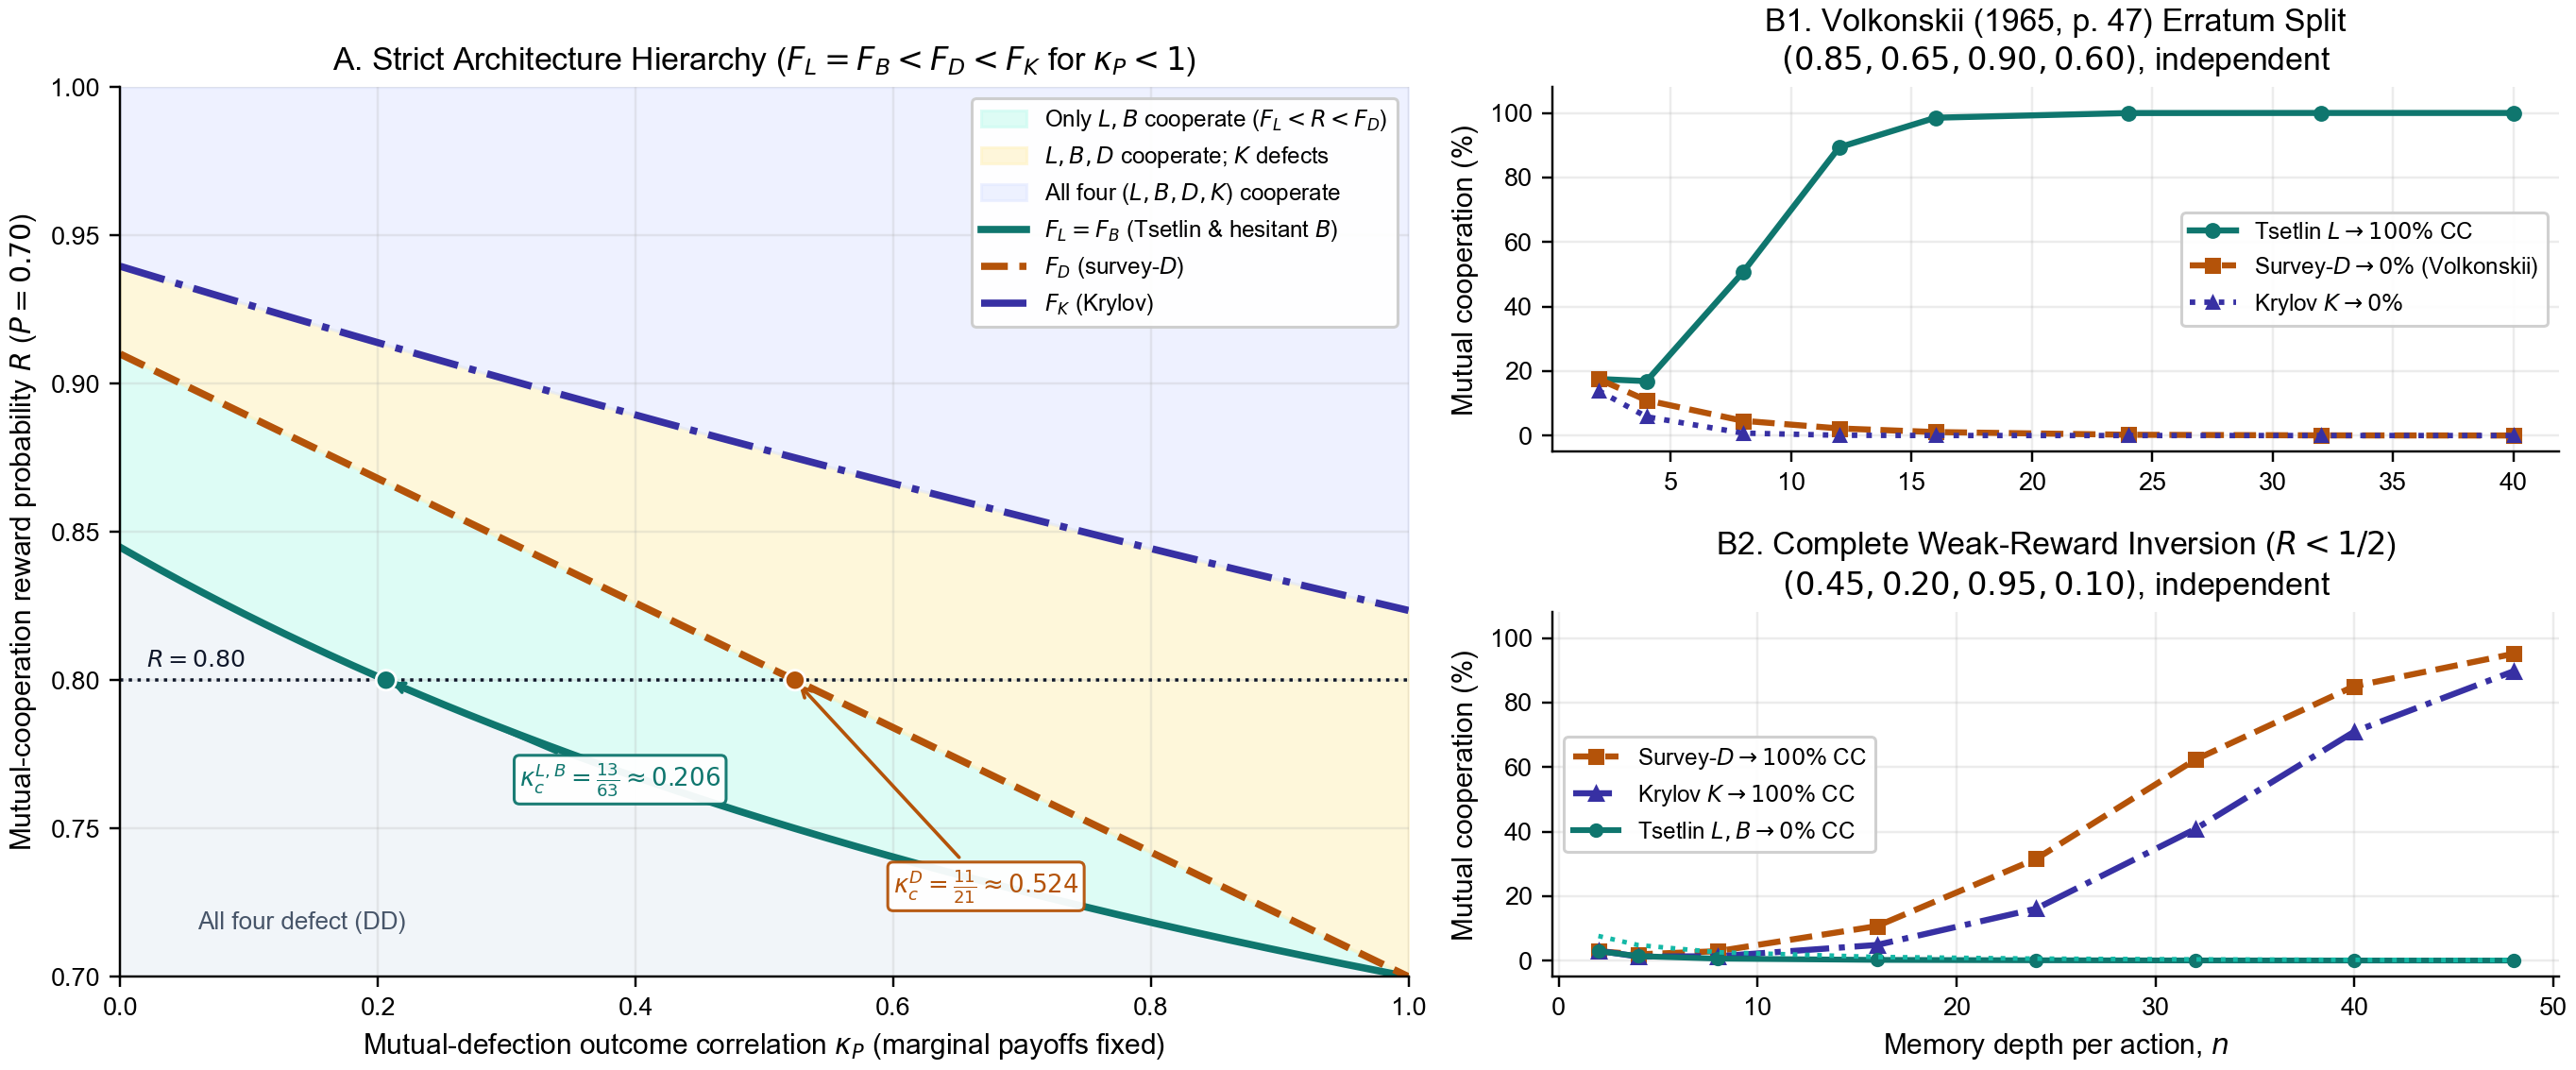
\includegraphics[width=\textwidth]{figs/p1_fig1_architecture_hierarchy.png}
  \caption{\textbf{Multi-architecture hierarchy, Volkonskii's 1965 erratum, and weak-reward inversion.}
  \textbf{(A)} Exact phase boundaries $F_L=F_B < F_D < F_K$ ($0 \le \kappa_P < 1$) at $P=0.70$, with critical correlations $\kappa_c^{L,B}=13/63$ and $\kappa_c^D=11/21$ along $R=0.80$ (where $K$ defects through $\kappa_P=1$).
  \textbf{(B1)} 80-digit GTH trajectories on Pyatetskii-Shapiro's benchmark $(0.85,0.65,0.90,0.60)$, $\kappa=0$: survey-$D$ collapses to $0\%$ as stated by Volkonskii \cite{Volkonskii1965}, whereas linear $L$ surges to $100\%$ ($\pi_{40}^L(CC)=0.99999991$), refuting the remark on p.~47 of \cite{Volkonskii1965}.
  \textbf{(B2)} Complete weak-reward reversal at $(0.45,0.20,0.95,0.10)$, $\kappa=0$ ($T+S=1.05>1$, $R>F_K>F_D$): $L,B \to (0,3/14,3/14,4/7)$ while survey-$D$ and Krylov $K$ converge to $100\%$ $CC$.}
  \label{fig:p1-hierarchy}
\end{figure}

\begin{remark}[Benchmarks and Volkonskii's 1965 Erratum]
In $(R, P, T, S) = (0.80, 0.70, 0.90, 0.20)$ at depth $n = 80$, 72-digit subtraction-free GTH elimination gives $\pi_{80}^L(CC) = 1.25 \times 10^{-12}$ at $\kappa_R = \kappa_P = 0$, versus $\pi_{80}^L(CC) = 0.9999999705$ at $\kappa_R = \kappa_P = 1/2$ (and $0.9999999666$ if $\kappa_R = 0, \kappa_P = 1/2$), which lies strictly above $\kappa_c^{L,B} = 13/63$, whereas survey-$D$ crosses to cooperation only strictly above $\kappa_c^D = 11/21$ (since $F_D(0.7, 1/2) = 0.805 > 0.80$) and $K$ remains in $DD$ even at $\kappa_P = 1$ ($F_K(0.7, 1) = 14/17 > 4/5$). On Pyatetskii-Shapiro's tuple $(0.85, 0.65, 0.90, 0.60)$ at $\kappa=0$, \eqref{eq:thresholds} yields
\[
  F_L(0.65, 0) = \frac{169}{218} \approx 0.7752 < R = \frac{17}{20} = 0.85 < \frac{351}{400} = 0.8775 = F_D(0.65, 0),
\]
producing opposite exponential slopes: $\pi_{40}^D(CC) = 1.02 \times 10^{-4}$ while $\pi_{40}^L(CC) = 0.99999991$ with exact log-odds slope $\log(833/507) \approx +0.4965$ (Figure~\ref{fig:p1-hierarchy}B1).
\end{remark}

\subsection{Complete Inversion in the Weak-Reward Regime (\texorpdfstring{$R < 1/2$}{R < 1/2})}
When all symmetric win probabilities fall below $1/2$, linear drift pushes $L$ and $B$ out of deep $CC$ and $DD$, inverting the hierarchy whenever $T + S \ge 1$ and $R$ lies above the $D, K$ thresholds.

\begin{theorem}[Weak-Reward Trichotomy and Complete Reversal]\label{thm:weak}
Suppose $0 < S < P < R < 1/2$ and $R < T < 1$, with independent mixed-profile feedback and full-support joint outcome laws at both symmetric profiles (arbitrary feasible correlations $\kappa_R, \kappa_P$). Define
\begin{equation}\label{eq:weak-params}
\begin{aligned}
  u &:= \frac{1-2P}{2(1-P-S)}, \qquad
  b := \frac{T-P}{1-P-S}, \qquad
  \mu := \frac{(1-2P)(T+S-1)}{1-P-S}, \\
  \sigma^2 &:= 8 u S(1-S) + 8(1-u) P(1-P)(1-\kappa_P) + \one_{\{B\}}\frac{(1-2P)(1-2S)}{1-P-S}.
\end{aligned}
\end{equation}
For equal-memory $L$ or $B$ automata as $n \to \infty$:
\begin{enumerate}
  \item \textbf{($T + S < 1$, i.e.\ $\mu < 0$)}: Both absolute depths have uniformly bounded exponential moments, and all four action profiles retain stationary probabilities bounded strictly away from $0$.
  \item \textbf{($T + S = 1$, i.e.\ $\mu = 0$)}: One player persists in $D$ with rescaled depth converging to $\mathrm{Uniform}[0,1]$, while the opponent converges to the two-sided geometric law $\nu(a,d) \propto \frac{1}{1-a}\bigl(\frac{a}{1-a}\bigr)^{d-1}$ ($a=S$ on $C$, $a=P$ on $D$), giving $\pi_n(CC) = \Theta(n^{-1})$ and limiting profile vector $(0,\, u/2,\, u/2,\, 1-u)$. Holding $R, P, S, \kappa_R, \kappa_P$ fixed and varying $T_n$ along $n(T_n + S - 1) \to a_0 \in \R$, the rescaled defector depth converges to density proportional to $e^{4 a_0 u x/\sigma^2}$ on $[0,1]$.
  \item \textbf{($T + S > 1$, i.e.\ $\mu > 0$)}: One player is pinned within a tight random distance of deepest $D$, the opponent converges to $\nu$, and $\pi_n \to (0,\, u/2,\, u/2,\, 1-u)$.
\end{enumerate}
Consequently, under the full-support hypotheses above (which for $p \in \{R, P\} < 1/2$ mean $-\frac{p}{1-p} < \kappa_p < 1$), whenever $T + S \ge 1$ and $R > F_K(P,\kappa_P) > F_D(P,\kappa_P)$ with $0 \le \kappa_P < 1$ (and for survey-$D$ at any full-support $\kappa_P$ whenever $R > F_D(P,\kappa_P)$), the architecture ordering inverts completely: $L$ and $B$ converge to $0\%$ mutual cooperation while survey-$D$ and Krylov $K$ converge exponentially to $(1, 0, 0, 0)$.
\end{theorem}

\begin{proof}[Proof outline]
Assign signed coordinates $y_i = \pm(d_i - 1/2)$ for $L$ and $y_i = \pm d_i$ for $B$ (positive on $D$, cap $M$). Letting $X = \max(y_1,y_2)$ and $Y = \min(y_1,y_2)$, since $P < R < 1/2$, both tails of $Y$ contract exponentially, yielding $\sup_n \E_{\pi_n}[e^{c|Y|}] \le C$. Freezing one player in $D$ gives the exact birth--death law $\nu$ with $\nu(C) = u$ and exact linear drift $\E[\Delta(x - b y) \mid x,y] = \mu$ away from the caps. When $\mu < 0$, $F = X - bY$ contracts outside a strip controlled by $|Y|$, yielding uniform exponential moments and full-support positive mass on all four profiles. When $\mu \ge 0$, $|y_1-y_2|$ is a submartingale with strict positive drift on an accessible set, ruling out any infinite-grid invariant probability; hence $X \to +\infty$ and $Y \Rightarrow \nu$, forcing $\pi_n \to (0,u/2,u/2,1-u)$. For $\mu > 0$, balancing $\Delta(X - bY)$ yields $\E_{\pi_n}[p_{\mathrm{high}}(Y)\one_{\{M-X=0\}}] \to \mu$, so any subsequential limit of $(G, Y) = (M-X, Y)$ has boundary flux $m\mu = \mu$, forcing total mass $m = 1$ and tightness of $M-X$. For $\mu = 0$, testing stationarity on $Z^2 = (y_1-y_2)^2$ bounds cap occupancy by $O(n^{-1})$, and testing the product $g(Z/n)v(Y)$ (bounded Lipschitz $g$, finitely supported $v$) forces every subsequential limit of $(Z/n, Y)$ to be a product $\lambda \otimes \nu$. Taylor-expanding stationarity of $n^2 f(Z/n)$ for smooth $f$ with Neumann conditions $f'(-1)=f'(1)=0$ yields $\frac{\sigma^2}{2}\int f''\,d\lambda = 0$, uniquely identifying the signed gap $Z/n \Rightarrow \mathrm{Uniform}[-1,1]$, whence $|Z|/n = X/n + o_P(1)$ gives $X/n \Rightarrow \mathrm{Uniform}[0,1]$. Along the $1/n$ window $n(T_n+S-1)\to a_0$, testing $W = |Z|/n$ against smooth unsigned Neumann functions $\phi$ ($\phi'(0)=\phi'(1)=0$) gives $\int (2a_0 u \phi' + \frac{\sigma^2}{2}\phi'')\,d\lambda_W = 0$, uniquely identifying density $\propto e^{4a_0 u x/\sigma^2}$ on $[0,1]$. Meanwhile, Theorem~\ref{thm:hierarchy} gives exponential $CC$ selection for $D$ (at any full-support $\kappa_P$ with $R > F_D$) and $K$ (for $0 \le \kappa_P < 1$ with $R > F_K$). On $(0.45,0.20,0.95,0.10)$ at $\kappa=0$, $T+S=1.05>1$, $u=3/7$, $F_D(0.2,0)=0.36 < F_K(0.2,0)=5/13 < 0.45$, yielding $L,B \to (0,3/14,3/14,4/7)$ vs.\ $\pi_{48}^D(CC)=95.1\%$, $\pi_{48}^K(CC)=89.7\%$ (Figure~\ref{fig:p1-hierarchy}B2).
\end{proof}

\section{Optimal Imperfect Correlation \texorpdfstring{$\kappa_*(\gamma)$}{kappa*(gamma)} and Interface Splitting}\label{sec:unequal}

Now let the two players possess unequal memory depths $n_1 \ge n_2 \ge 1$ with $n_1/n_2 \to \gamma > 1$, under $0 < S \le 1/2 < P < R < T < 1$, independent mixed-profile feedback, arbitrary feasible $\kappa_R$, and variable $DD$ correlation $\kappa_P$. Denote the deepest joint states by $K_D, K_C$, and define the lower limiting escape cost per unit of short memory:
\[
  \underline{V}(\gamma, \kappa_P) := \liminf_{n_2 \to \infty} \Bigl(-\frac{1}{n_2}\log \Prob_{K_D}(\tau_{K_C} < \tau_{K_D}^+)\Bigr).
\]
(Theorem~\ref{thm:interface} establishes that the ordinary limit $V(\gamma,\kappa_P)$ exists globally for $L$ across all feasible $\kappa_P$, and for $B$ on all $0 \le \kappa_P \le 1$ as well as the negative-correlation subregions $h \le h_T$ or $-\frac{1}{2}\log\frac{S}{1-S} \le \log(2-e^{-h_P})$.) Let $h_P = \log\frac{P}{1-P}$, $h_R = \log\frac{R}{1-R}$, $h_T = \log\frac{T}{1-T}$, and $\delta = 2P-1$.

\begin{theorem}[Unique Payoff-Independent Optimal Correlation and Quadratic Expansion]\label{thm:optimal-corr}
For both Tsetlin $L$ and randomized-boundary $B$, the global minimum of $\underline{V}(\gamma, \kappa_P)$ over all feasible $\kappa_P$ equals $\gamma h_P$ (attained as a true limit $V = \gamma h_P$), and is attained at the \emph{unique}, payoff-independent imperfect correlation
\begin{equation}\label{eq:kstar}
  \kappa_*(\gamma) = \frac{1 + 1/\gamma}{2} \in \Bigl(\frac{1}{2}, 1\Bigr).
\end{equation}
Consequently, the supremum aspect ratio permitting strict exponential cooperation is $\gamma_{\max} = h_R / h_P$ (strict cooperation holds for $\gamma < \gamma_{\max}$ near $\kappa_*(\gamma)$, while at $\gamma = \gamma_{\max}$ the rates tie at $\kappa_*(\gamma_{\max}) = \frac{1+h_P/h_R}{2}$). At fixed $\gamma > 1$, $V(\gamma,\kappa)$ is smooth near $\kappa_*(\gamma)$ for both $L$ and $B$ with exact quadratic expansion (second derivative $2 C_\gamma$)
\begin{equation}\label{eq:curvature}
  V(\gamma, \kappa) = \gamma h_P + C_\gamma (\kappa - \kappa_*(\gamma))^2 + O(|\kappa - \kappa_*(\gamma)|^3), \qquad
  C_\gamma := \frac{2\gamma\delta}{(1 - 1/\gamma)(1 + \delta^2/\gamma)} > 0,
\end{equation}
yielding leading-order symmetric square-root tip closure $\kappa_\pm(\gamma) = \kappa_*(\gamma) \pm \sqrt{(h_R - \gamma h_P)/C_\gamma} + O(h_R - \gamma h_P)$ as $\gamma \uparrow \gamma_{\max}$.
\end{theorem}

\begin{proof}
Because player 1 must make a first action switch from $K_D$ while its erosion probability in $DD$ is $1-P$ (and $B$ can only decline switches), one-coordinate gambler's ruin over the polynomial excursion window gives $\underline{V}(\gamma,\kappa_P) \ge \gamma h_P$ for every feasible $\kappa_P$. Write the $DD$ and mixed moment generating functions (with $s$ tilting the long coordinate and $t$ the short coordinate, positive toward cooperation) as
\begin{equation}\label{eq:MGF-DC}
  D(s,t) = A_P e^{-s-t} + C_P(e^{s-t} + e^{-s+t}) + B_P e^{s+t}, \qquad
  C(s,t) = \bigl(T e^{-s} + (1-T)e^s\bigr)\bigl(S e^t + (1-S)e^{-t}\bigr).
\end{equation}
At the natural long-player tilt $(s,t) = (h_P, 0)$, we have $D(h_P,0) = 1$, tilted long-coordinate mean $\E_*[U] = \delta > 0$, and tilted short-coordinate mean $\E_*[V_2] = \delta(2\kappa_P - 1)$. The ratio of tilted speeds matches $\gamma$ precisely when $\gamma(2\kappa_P - 1) = 1$, i.e.\ $\kappa_P = \kappa_*(\gamma)$, where the straight tilted path stays inside $DD$ until simultaneous switching and realizes $V = \gamma h_P$.

For strictness away from $\kappa_*(\gamma)$: along $D(s(t), t) = 1$ through $(h_P, 0)$, implicit differentiation yields $s'(0) = -(2\kappa_P - 1)$ and $\left.\frac{d}{dt}(\gamma s(t) + t)\right|_{t=0} = 1 - \gamma(2\kappa_P - 1)$. For $\kappa_P \in [1/2, \kappa_*)$, small $t > 0$ strictly raises $\gamma s(t) + t$; for $\kappa_P \in (\kappa_*, 1)$, small $t < 0$ strictly raises $\gamma s(t) + t$ while both $C(h_P,0) = T e^{-h_P} + (1-T)e^{h_P} < 1$ (since $T > P$) and the randomized-boundary constraint stay strictly slack. For $0 \le \kappa_P < 1/2$, $D_t(h_P,0) < 0$ allows positive $t$; for $\kappa_P < 0$, the negative-shock decomposition gives a strict positive offset over $\gamma h_P$; and at $\kappa_P = 1$, Theorem~\ref{thm:interface} yields $V = h_P + (\gamma - 1)s_{I,u} > \gamma h_P$ since $s_{I,u} > h_P$.

For \eqref{eq:curvature}, set $w = 2\kappa_P - 1$. Under the $(h_P,0)$ tilt, conditional regression gives $D_2 := \E_*[(V_2 - w U)^2] = (1-w)(1 + w\delta^2)$, so $s''(0) = -D_2/\delta$. Maximizing $\gamma h_P + (1-\gamma w)t - \frac{\gamma D_2}{2\delta} t^2 + O(t^3)$ over $t$ evaluates the quadratic coefficient at $w = 1/\gamma$ to $C_\gamma = \frac{2\gamma\delta}{(1-1/\gamma)(1+\delta^2/\gamma)}$.
\end{proof}

\begin{remark}[Contrast with Brownian Ruin]
In two-dimensional equal-capital unequal-drift Brownian ruin, Debicki, Ji, and Rolski \cite{DJR2019} obtain $(1+\mu_1/\mu_2)/2$ as the boundary of a \emph{flat} rate plateau. In our discrete-lattice action-switching automata game, $\kappa_*(\gamma) = (1+1/\gamma)/2$ is instead a \emph{strict unique minimizer} with positive quadratic coefficient $C_\gamma$, whose cooperation domain closes symmetrically to leading order near $\gamma_{\max}$ and collapses at both extremes ($\kappa_P = 0$ and $\kappa_P = 1$) whenever $\gamma$ exceeds both endpoint critical aspect ratios (for instance at $\gamma = 3$ in Corollary~\ref{cor:showcase}, whereas small ratios such as $\gamma = 1.1$ remain cooperative at both endpoints).
\end{remark}

\subsection{Interface Splitting: How Doorway Hesitation (\texorpdfstring{$B$}{B}) Beats Linear (\texorpdfstring{$L$}{L})}
When $1/2 < \kappa_P \le 1$ and $\gamma(2\kappa_P - 1) > 1$, the unconstrained $DD$ bulk optimum may either stay slack at the mixed boundary or violate it; in the active case, the short-memory player reaches its switching interface early and oscillates across the $DD$/mixed boundary while the long player inches toward $C$. Let $A_D(s) := B_P e^s + C_P e^{-s}$, $B_D(s) := C_P e^s + A_P e^{-s}$ ($D = A_D e^t + B_D e^{-t}$), $m_T(s) := T e^{-s} + (1-T)e^s$, $A_C(s) := S m_T(s)$, and $B_C(s) := (1-S) m_T(s)$. Denote by $z_D(s)$ the larger positive root of $A_D(s) z^2 - z + B_D(s) = 0$ (on $4A_D(s)B_D(s) \le 1$) and by $z_C(s)$ the smaller positive root of $A_C(s) z^2 - z + B_C(s) = 0$.

\begin{theorem}[Action-Switching Interface Rate and M\"obius Splitting]\label{thm:interface}
Assume $0 < S \le 1/2 < P < R < T < 1$, $n_1/n_2 \to \gamma \ge 1$, independent mixed-profile feedback, arbitrary feasible $\kappa_R$, and weak-loss exit switch probability $u \in (0,1]$ ($L$: $u=1$; $B$: $u=1/2$). Define the M\"obius return operator (extended continuously to $\Phi_u(1) = 1$)
\begin{equation}\label{eq:mobius}
  \Phi_u(z) := (1 - u) + \frac{u^2 z}{1 - (1-u)z}, \qquad z \in (0,1].
\end{equation}
In each of the following proved cases, $\pi_{n_1,n_2}(CD)+\pi_{n_1,n_2}(DC)\to 0$ and
\[
  \lim_{n_2\to\infty}\frac{1}{n_2}\log\frac{\pi_{n_1,n_2}(CC)}{\pi_{n_1,n_2}(DD)} = h_R - V_u,
\]
where:
\begin{enumerate}
  \item If $0 \le \kappa_P < 1$ and $\gamma(2\kappa_P - 1) \le 1$, then $V_u = \max\{\gamma s + t : 0 \le s,t \le h_P,\, D(s,t)\le 1\}$ (independent of $u$; in particular $V_u = (\gamma+1)h_P$ at $\kappa_P=0$).
  \item If $1/2 < \kappa_P < 1$ and $\gamma(2\kappa_P - 1) > 1$, then
  \begin{equation}\label{eq:Vu}
    V_u = \max_{s}\Bigl\{\gamma s + \log z_D(s) : h_P \le s \le h_T,\;\; 4A_D(s)B_D(s) \le 1,\;\; z_D(s) \ge \Phi_u(z_C(s))\Bigr\}.
  \end{equation}
  \item If $\kappa_P = 1$: at $\gamma = 1$, $V_u = h_P$ for every $u \in (0,1]$; for $\gamma > 1$, $V_u = h_P + (\gamma - 1) s_{I,u}$, where $s_{I,u} > h_P$ is the unique root of $e^{h_P - s} = \Phi_u(z_C(s))$, giving $\gamma_c^{(u)} = 1 + (h_R - h_P)/s_{I,u}$.
  \item If $\kappa_P < 0$: let $h := \sup\{v \ge 0 : \min_{s \ge h_P} D(s,v) \le 1\}$ (with $h = +\infty$ at $B_P = 0$). For $S = 1/2$, $V_u = \gamma h_P + \min(h, h_T)$ for both $L$ and $B$. For $S < 1/2$, let $v_m > h_T$ be the larger root of $m_T(v_m) = \bigl(2\sqrt{S(1-S)}\bigr)^{-1}$; then $V_L = \gamma h_P + \min(h, v_m)$ globally for $L$, and the same formula holds for $B$ whenever $h \le h_T$ or $-\frac{1}{2}\log\frac{S}{1-S} \le \log(2 - e^{-h_P})$.
\end{enumerate}
Because $\Phi_u(z)$ decreases strictly with $u \in (0,1]$ on $(0,1)$ ($\Phi_1(z)=z < \Phi_{1/2}(z) = \frac{1}{2-z}$), lowering $u$ raises $\Phi_u(z_C(s))$ and tightens $z_D(s) \ge \Phi_u(z_C(s))$, shrinking the feasible interval of $s$ in \eqref{eq:Vu}; whenever the mixed constraint strictly reduces the maximum, we obtain strict phase splitting $V_B < V_L$, so hesitant $B$ selects $CC$ across an open band of $(R, \kappa_P, \gamma)$ where linear $L$ selects $DD$.
\end{theorem}

\begin{proof}[Proof outline]
For the upper bound on escape probability in Cases (2)--(3), place $k=0$ at the short player's shallow $D$ state and $k=1$ at its shallow $C$ state. In the infinite $C$ half-line, the $m_T(s)$-discounted return transform from $k=1$ to $k=0$ solves $g_C = u z_C / (1 - (1-u)z_C)$, so a step into the weak $C$ interface from $k=0$ yields return weight $(1-u) + u g_C = \Phi_u(z_C(s))$. Whenever $z_D(s) \ge \Phi_u(z_C(s))$, splicing $e^{t_D(s) y}$ on $DD$ with a finite-cap perturbation of the $m_T(s)$-harmonic function on $C$ constructs a positive supermartingale $e^{s X} f_n(Y)$ while the long player stays in $D$, proving $\underline{V}_u \ge \gamma s + \log z_D(s)$ (with $O(n^2)$ regeneration blocks and an $n^4$ cutoff at $S = 1/2$). For the matching lower bound when the interface constraint strictly truncates the bulk optimizer at $s_{I,u}$ (at first contact with the bulk optimizer, the direct interior path already achieves the rate), define the first-return transform $\mathcal{R}_u(s) := B_D(s)/z_D(s) + A_D(s)\Phi_u(z_C(s))$, which satisfies $\mathcal{R}_u(s_{I,u}) = 1$ since $z_D(s_{I,u}) = \Phi_u(z_C(s_{I,u}))$. Differentiating $\mathcal{R}_u$ at $s_{I,u}$ shows $\mathcal{R}_u'(s_{I,u}) > 0$ (accounting automatically for boundary holds when $u < 1$), proving strictly positive longitudinal drift $\bar v_x > 0$ per return cycle of the positive-recurrent tilted strip and telescoping the likelihood ratio to $s_{I,u} n_1 + \log z_D(s_{I,u}) n_2 + o(n_2)$. Case (4) follows from the negative-shock last-departure decomposition (\texttt{docs/phase1\_negative\_krylov.md}).
\end{proof}

\begin{figure}[t]
  \centering
  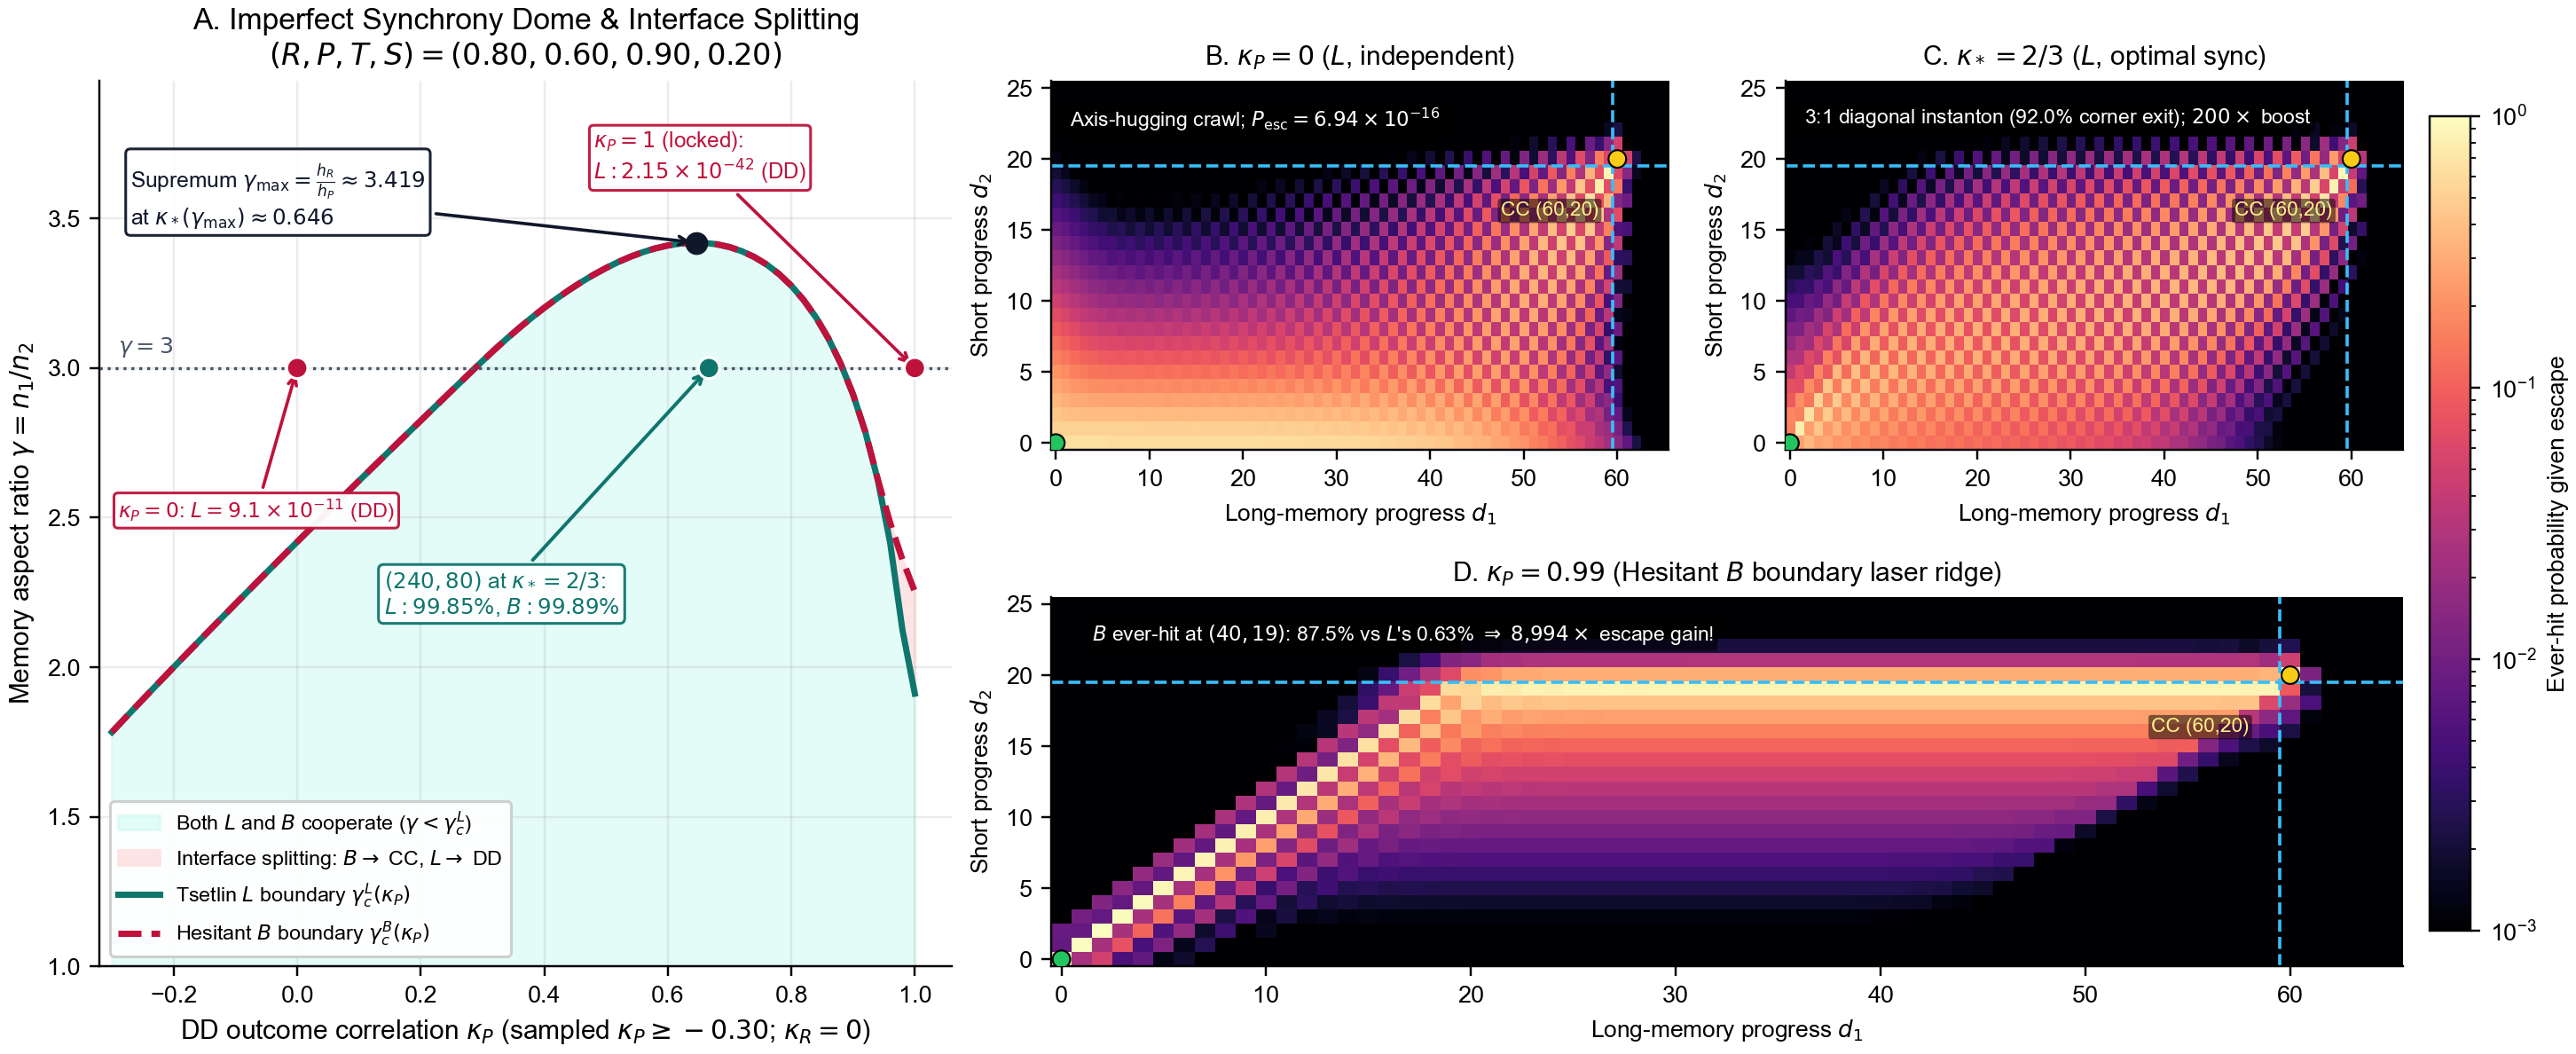
\includegraphics[width=\textwidth]{figs/p1_fig2_unequal_escape_instanton.png}
  \caption{\textbf{Imperfect synchrony dome, interface splitting, and instanton anatomy in $(0.80,0.60,0.90,0.20)$.}
  \textbf{(A)} Critical aspect ratio $\gamma_c(\kappa_P)$ (sampled $\kappa_P \ge -0.30$) with supremum $\gamma_{\max}=h_R/h_P \approx 3.419$ at $\kappa_* \approx 0.646$, certified $(240,80)$ $L$ stationary masses flipping $9.08\times 10^{-11} \to 99.85\% \to 2.15\times 10^{-42}$ across $\kappa_P = 0 \to 2/3 \to 1$, and the $B$-beats-$L$ splitting wedge near $\kappa_P=1$.
  \textbf{(B--D)} 75-digit conditional ever-hit probability heatmaps on the $(60,20)$ memory rectangle: axis-hugging crawl at $\kappa_P=0$ ($P_{\mathrm{esc}}=6.94\times 10^{-16}$), straight $3:1$ diagonal instanton at $\kappa_*=2/3$ ($92.0\%$ terminal entry at $(60,20)$, $36.85\%$ simultaneous first switches, $200\times$ boost), and hesitant $B$'s boundary laser ridge at $\kappa_P=0.99$ (ever-hit probability $87.48\%$ vs.\ $0.63\%$ for $L$ at $(40,19)$, yielding an $8{,}994.22\times$ escape gain).}
  \label{fig:p1-instanton}
\end{figure}

\begin{corollary}[Certified $DD$--$CC$--$DD$ Flip Interval and $8{,}994\times$ Amplification]\label{cor:showcase}
Fix $(P,T,S)=(0.60,0.90,0.20)$ and $\gamma=3$ ($h_P = \log(3/2)$). For every $R \in (27/35,\, 81/97)$, both $L$ and $B$ select $DD$ at $\kappa_P=0$ ($V=4h_P$) and at $\kappa_P=1$, yet select $CC$ at $\kappa_* = 2/3$ ($V=3h_P$). Indeed, at $\kappa_P=1$ the feasible tilt $s = \log 2$ gives $z_D = 3/4$ and mixed polynomial $(13/100)z^2 - z + 13/25 = 0$ (smaller root $z_C < 2/3$, hence $\Phi_{1/2}(z_C) = \frac{1}{2-z_C} < 3/4$), certifying $V_L > V_B \ge h_P + 2\log 2 = \log 6 > 4 h_P$. At $R=0.80, \kappa_R=0$ (76-digit rational Poisson enclosures, Table~\ref{tab:showcase}), $(240,80)$ flips $9.084\times 10^{-11} \to 99.8529\% \to 2.150\times 10^{-42}$ for $L$. At $(0.78,0.60,0.90,0.20, \kappa_P=0.99, \gamma=2)$, $V_B = 1.15386 < h_R = 1.26567 < V_L = 1.38349$ ($B\to 100\%$ $CC$, $L\to 100\%$ $DD$). At $(60,20), R=0.80, \kappa_P=0.99$, $B$'s per-excursion escape probability is $8{,}994.22\times$ $L$'s ($1.418\times 10^{-18}$ vs.\ $1.577\times 10^{-22}$), with conditional ever-hit probability $87.48\%$ (mean $1.817$ visits) vs.\ $0.63\%$ ($0.021$ visits) at $(40,19)$ and $30.73$ mean declined shallow losses (Figure~\ref{fig:p1-instanton}D).
\end{corollary}

\begin{table}[t]
\centering
\caption{Certified 76-digit stationary cooperation probabilities $\pi_{n_1,n_2}(CC)$ for $(R,0.60,0.90,0.20)$, $\gamma=3$, $\kappa_R=0$.}
\label{tab:showcase}
\begin{tabular}{@{}lllrrr@{}}
\toprule
$R$ & Depths $(n_1,n_2)$ & Architecture & $\kappa_P = 0$ & $\kappa_P = 2/3$ & $\kappa_P = 1$ \\
\midrule
$0.80$ & $(240,80)$ & Tsetlin $L$ & $9.0843 \times 10^{-11}$ & $0.99852907$ & $2.1501 \times 10^{-42}$ \\
$0.80$ & $(240,80)$ & Hesitant $B$ & $9.7114 \times 10^{-11}$ & $0.99894320$ & $3.4878 \times 10^{-22}$ \\
$0.82$ & $(150,50)$ & Tsetlin $L$ & $6.8843 \times 10^{-5}$ & $0.99970439$ & $2.4836 \times 10^{-24}$ \\
$0.82$ & $(150,50)$ & Hesitant $B$ & $7.2667 \times 10^{-5}$ & $0.99978860$ & $9.5019 \times 10^{-12}$ \\
\bottomrule
\end{tabular}
\end{table}

\section{2D Correlated Quadrant Trichotomy and Fair-DD Elliptic Cancellation}

\subsection{Exact Four-Regime Classification of the Stopped Correlated Quadrant}
Consider the frozen symmetric $DD$ walk $(X_t, Y_t)$ on $\Z_{\ge 0}^2$ with reflection $X' = \max(0, X+U)$, $Y' = \max(0, Y+V)$, starting at $(0,0)$, with increments $(+1,+1), (+1,-1), (-1,+1), (-1,-1)$ having probabilities $(B_p, C_p, C_p, A_p)$ for $1/2 < p < 1$ and $-q/p < \kappa < 1$. Let $h_{m,n}$ be the probability of hitting $(m,n)$ before returning positively to $(0,0)$ or overflowing $X > m$ or $Y > n$. Set $M(s,t) = B_p e^{s+t} + 2 C_p \cosh(s-t) + A_p e^{-s-t}$ and $H(x,y) = \max_{M(s,t)\le 1} (sx + ty)$.

\begin{theorem}[2D Correlated Quadrant Trichotomy]\label{thm:quadrant}
Fix $1/2 < p < 1$, $-q/p < \kappa < 1$, $\gamma \ge 1$, and $m = \gamma n + O(1)$. Set $\delta = 2p-1$, $r = \log(p/q)$, and for $\kappa < 1/2$:
\[
  \lambda = 1 - 2\kappa, \qquad
  t_* = \log\frac{1 + \delta\lambda}{1 - \delta\lambda}, \qquad
  g(\delta,\lambda) = \frac{1 + (1-\delta^2)\lambda - \lambda^2}{\lambda(1 - \delta^2\lambda^2)}.
\]
Then $h_{m,n} = \Theta(n^\beta e^{-n E})$, partitioned into exactly four regimes:
\begin{center}
\small
\begin{tabular}{@{}llll@{}}
\toprule
Parameter regime & Rate $E$ & $\beta$ & Optimal macroscopic route \\
\midrule
$\kappa \ge 1/2$, or ($\kappa < 1/2$, $g > \gamma$) & $H(\gamma,1)$ & $-1/2$ & Direct oblique interior path \\
$\kappa < 1/2$ and $0 < g \le \gamma$ & $r\gamma + t_*$ & $0$ & Long axis, then oblique slope $g:1$ \\
$\kappa < 1/2$ and $g = 0$ & $r\gamma + t_*$ & $-1/2$ & Long axis, then zero-horizontal-drift leg \\
$\kappa < 1/2$ and $g < 0$ & $r\gamma + H(0,1)$ & $-3/2$ & Ceiling-ballot leg left of $X=m$ \\
\bottomrule
\end{tabular}
\end{center}
Explicitly, $H(x,y) = u(x+y)/2 + v|x-y|/2$ where, setting $\eta = |x-y|/(x+y)$, $e=\eta^2$, $c=4C_p^2 + e(1-4A_p B_p)$, and $z = c/(e + \sqrt{e^2 + (1-e)c})$,
\[
  u = \log\frac{1 - z + \sqrt{(1-z)^2 - 4 A_p B_p}}{2 B_p}, \qquad
  v = \arcosh\frac{z}{2 C_p}.
\]
In particular, along the diagonal $m=n$, $0 < \kappa < 1$ gives $E = \log(A_p/B_p)$ with $\beta = -1/2$, while $\kappa = 0$ gives $E = 2r$ with $\beta = 0$ (whose exact boundary denominator is the squared-Catalan-number series $\sum_{j\ge 0} C_j^2 (pq)^{2j}$). Within the negative-correlation interval $-q/p < \kappa < 0$, the transition $g=0$ occurs at $\lambda_0 = \frac{1-\delta^2 + \sqrt{(1-\delta^2)^2 + 4}}{2}$, separating $\beta \in \{0, -1/2, -3/2\}$ across $\kappa \gtreqless \kappa_0 = (1-\lambda_0)/2$. At $\kappa = -q/p$ ($B_p = 0$), $h_{m,n} = 0$ for all $m,n\ge 1$; at $\kappa = 1$, $h_{m,n} = 0$ for $m>n$ and $h_{n,n} = q(e^r-1)/(e^{rn}-1)$.
\end{theorem}

\begin{proof}[Proof outline]
Exponential tilting by the harmonic tilt $(s,t)$ on $\{M=1\}$ converts the stopped walk into a drifted/zero-drift 2D walk killed at $\{X>m\} \cup \{Y>n\} \cup \{(0,0)\}$. In the direct interior regime, the 2D local CLT along the straight line to $(m,n)$ gives a single transverse Gaussian constraint $\Theta(n^{-1/2})$. When $0 < g \le \gamma$, the path rides the $X$-axis (cost $r$ per step) and launches from $X_0 = m - g n + O(\sqrt{n})$, whose $\Theta(\sqrt{n})$ launch window cancels $n^{-1/2}$ to yield $\beta = 0$. At $g=0$, the launch sits at distance $\Theta(\sqrt{n})$ from $X=m$ with half-line killing, leaving $\beta = -1/2$. When $g < 0$, the competing axis tilt $(r, t_*)$ has negative horizontal drift, so the maximizing tilt $(s_0, t_0)$ attaining $H(0,1)$ sits at the vertical support point with $s_0 > r$ and \emph{zero} horizontal drift; weighting each departure at deficit $\ell = m - X_0$ by $e^{-(s_0-r)\ell}$ and applying the ballot/reflection factor $2(\ell+1)/(j+\ell+2)$ for staying at or below $X=m$ before hitting $(m,n)$ at step $j$ supplies an additional $O(n^{-1})$ survival factor, yielding $\beta = -3/2$.
\end{proof}

\subsection{Direct Interacting-Game Observables at Fair \texorpdfstring{$DD$ ($P=1/2$)}{DD (P=1/2)} and Three-Way Elliptic Cancellation}
Now set $P = 1/2$ with independent $DD$ feedback and arbitrary $R, S, T$ ($M \ge N \ge 1$ memory states per action). Restrict the actual two-player game transition matrix to the $MN$ states of $DD$ to obtain the symmetric substochastic matrix $K$ and Green matrix $G = (I - K)^{-1}$ (including time $0$), with deepest state $o = (0,0)$ and joint shallow doorway $c = (M-1, N-1)$. Let $w \in \{0, 1/4\}$ be the shallow hold probability ($w=0, a=1/2$ for $L$; $w=1/4, a=1/4$ for $B$, where $a = 1/2 - w$). Write $\sigma$ for the first exit from $DD$ and $\zeta$ for the first positive return to $o$. Define:
\begin{itemize}
  \item $h$: probability of visiting $c$ at least once during an origin excursion (ending at $\sigma \wedge \zeta$);
  \item $j_{\mathrm{imm}} := h a^2$: probability per excursion of reaching $c$ and switching together to $CC$ on the \emph{very next round} (conditional on arrival at $c$, the switch ratio $a_B^2/a_L^2$ is $1/4$);
  \item $d$ (resp.\ $b$): probability of a clean zero-betrayal transition $DD \to CC$ during a single origin excursion (resp.\ at the first exit $\sigma$ from $DD$, allowing arbitrary returns to $o$).
\end{itemize}

\begin{theorem}[Exact Green Identities, Three-Way Cancellation, and Universal Elliptic Laws]\label{thm:fair-elliptic}
For every finite memory pair $M \ge N \ge 1$ ($c \neq o$ for $h, V$):
\begin{equation}\label{eq:green-identities}
\begin{aligned}
  b &= a^2 G_{oc}, \qquad
  d = \frac{b}{G_{oo}} = a^2 \frac{G_{oc}}{G_{oo}}, \qquad
  \Prob_o(\sigma < \zeta) = \frac{1}{G_{oo}}, \\
  V &:= G_{cc} - \frac{G_{oc}^2}{G_{oo}}, \qquad
  h = \frac{G_{oc}}{G_{oo} V}, \qquad
  d = h\, a^2 V.
\end{aligned}
\end{equation}
As $N \to \infty$ with $M/N \to \gamma \in [1,\infty)$, let $D_0 := \frac{16}{\pi} - 4$, $D_{1/4} := \frac{16}{5}\bigl(\frac{4\log 3}{\pi} - 1\bigr)$, and define the universal elliptic shape factor
\begin{equation}\label{eq:I-gamma}
  I(\gamma) := 2\pi \sum_{k=0}^\infty \frac{(-1)^k (2k+1)}{\cosh\bigl((2k+1)\pi\gamma/2\bigr)}
  = \frac{4 k k' K(k)^2}{\pi} \qquad \Bigl(\frac{K(k')}{K(k)} = \gamma\Bigr).
\end{equation}
Then $G_{oc} \sim \frac{I(\gamma)}{(1-2w)^2 N^2}$, $G_{oo} \sim \frac{4}{\pi}\log N$, and $G_{cc} \to D_w$, producing:
\begin{enumerate}
  \item \textbf{Three-Way Limiting Architecture Cancellation}: Across every aspect ratio $\gamma \ge 1$, the limiting $B/L$ ratios satisfy
  \begin{align*}
    \frac{h_B}{h_L} &\longrightarrow \frac{4 D_0}{D_{1/4}} = \frac{5(4-\pi)}{4\log 3 - \pi} \approx 3.42580074, &
    \frac{j_{\mathrm{imm}}^B}{j_{\mathrm{imm}}^L} &\longrightarrow \frac{D_0}{D_{1/4}} \approx 0.85645019, \\
    \frac{d_B}{d_L} &\longrightarrow 1, &
    \frac{b_B}{b_L} &\longrightarrow 1.
  \end{align*}
  (At finite depth the ratios differ---e.g.\ $d_B/d_L = 1/4$ at $M=N=1$, converging to $0.999484$ at $M=N=4096$ and $1.000251$ at $M=3N=12288$.)
  \item \textbf{Universal Elliptic Breakout Laws}: For \emph{both} $L$ and $B$ identically,
  \begin{equation}\label{eq:elliptic-laws}
    d \sim \frac{\pi I(\gamma)}{16 N^2 \log N}, \qquad
    b \sim \frac{I(\gamma)}{4 N^2},
  \end{equation}
  with square ($\gamma=1$) constants $\frac{\Gamma(1/4)^4}{128\pi} \approx 0.42969911$ and $\frac{\Gamma(1/4)^4}{32\pi^2} \approx 0.54710990$.
  \item \textbf{First-Exit Waiting Time and Long-First Probability}: Setting $r_k = 2k+1$,
  \[
    \E_o[\sigma] \sim K(\gamma) N^2, \qquad
    \Prob_o(\text{long switches alone at }\sigma) \longrightarrow J(\gamma),
  \]
  where $K(\gamma) = 1 - \frac{32}{\pi^3}\sum_{k\ge 0}\frac{(-1)^k}{r_k^3 \cosh(r_k\pi\gamma/2)}$ and $J(\gamma) = \frac{4}{\pi}\sum_{k\ge 0}\frac{(-1)^k}{r_k \cosh(r_k\pi\gamma/2)}$ ($K(1) \approx 0.589371$, $J(1) = 1/2$; $K(3) \approx 0.981459$, $J(3) \approx 0.022873$).
\end{enumerate}
\end{theorem}

\begin{proof}[Proof outline]
Because only $c$ admits a direct transition to $CC$ (with probability $a^2$), summing over visits to $c$ before $\sigma$ gives $b = a^2 G_{oc}$; renewal at $o$ gives $G_{oo}$ expected excursion starts, proving $d = b/G_{oo}$ and $\Prob_o(\sigma<\zeta) = 1/G_{oo}$. Decomposing $G_{oc}$ at the first visit to $c$ and subtracting paths returning to $o$ before revisiting $c$ gives $V = G_{cc} - G_{oc}^2/G_{oo}$ and $d = h a^2 V$.

Since the players evolve independently inside $DD$ until $\sigma$, $K$ is the tensor product of two 1D substochastic transition matrices on $\{0,\dots,M-1\}$ and $\{0,\dots,N-1\}$. Diagonalizing via the exact discrete cosine eigenbases gives $G_{oc} \sim I(\gamma)/((1-2w)^2 N^2)$, $G_{oo} \sim \frac{4}{\pi}\log N$, and $G_{cc} \to D_w$. Because $1-2w = 2a$, $a^2$ cancels $(1-2w)^{-2}$ identically in the leading terms of $b = a^2 G_{oc}$ and $d = b/G_{oo}$: symbolically, $\frac{4 D_0}{D_{1/4}} \cdot \frac{1}{4} \cdot \frac{D_{1/4}}{D_0} = 1$ (Figure~\ref{fig:p1-fair}). Finally, coupling up to $\sigma$ identifies $\sigma \stackrel{d}{=} \min(\tau_M, \tau_N)$ with independent 1D exit times. For $L$, the exact generating function from $0$ is $\E[z^{\tau_N}] = \cosh(\xi/2)/\cosh((N+1/2)\xi)$ ($\cosh\xi=1/z$), whose diffusive limit $\tau_N/N^2 \Rightarrow \tau$ is standard Brownian exit from $(-1,1)$. For $B$, the trajectory agrees with $L$ until its first shallow hit, after which its remaining mean exit time is $N/a = 4N = o(N^2)$ (vs.\ $2N$ for $L$), so both architectures share the same diffusive limit $\tau$ with uniform exponential tails, producing $K(\gamma)$ and $J(\gamma)$ via $\Prob(\tau > t) = \sum_{k\ge 0} \frac{4(-1)^k}{\pi r_k} e^{-\pi^2 r_k^2 t/8}$.
\end{proof}

\begin{figure}[t]
  \centering
  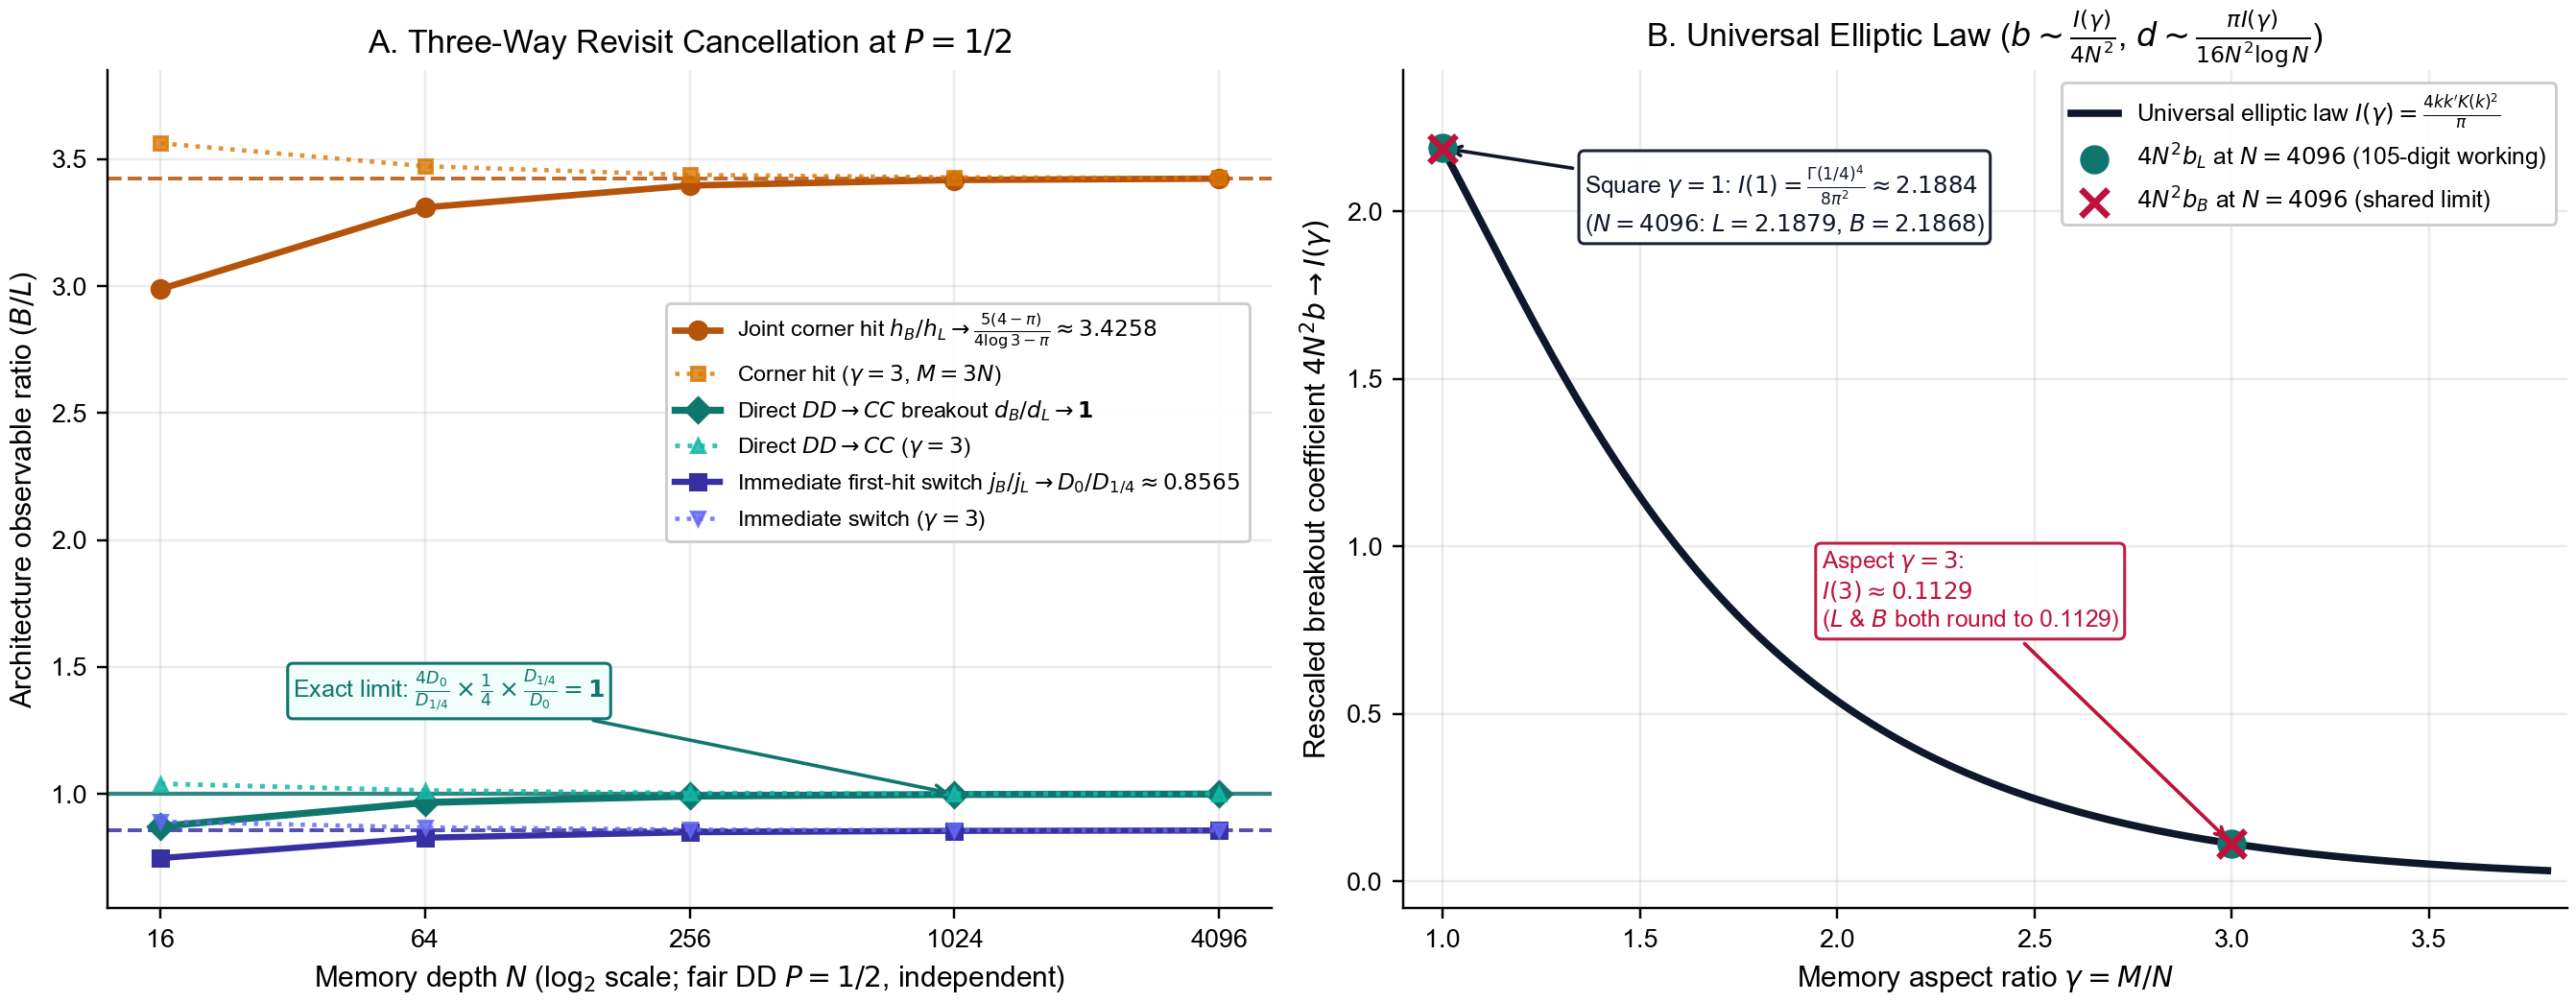
\includegraphics[width=\textwidth]{figs/p1_fig3_fair_elliptic_cancellation.png}
  \caption{\textbf{Three-way revisit cancellation and universal elliptic breakout law at fair $DD$ ($P=1/2$, independent).}
  \textbf{(A)} Spectral ratios $B/L$ (105-digit working, 82-digit exported) for $N = 16 \dots 4096$ at $\gamma = 1$ and $\gamma = 3$: joint corner hits converge to $\frac{5(4-\pi)}{4\log 3 - \pi} \approx 3.4258$, immediate switches to $0.8565$, while extra revisits ($D_{1/4}/D_0$) cancel the direct zero-betrayal $DD \to CC$ breakout ratio to $1$ in the limit ($0.99948$ at $N=4096, \gamma=1$; $1.00025$ at $\gamma=3$).
  \textbf{(B)} Universal elliptic curve $I(\gamma) = \frac{4kk'K(k)^2}{\pi}$ compared against $4N^2 b_L$ and $4N^2 b_B$ at $N=4096$: at $\gamma=1$, $I(1) \approx 2.1884$ ($L$: $2.1879$, $B$: $2.1868$); at $\gamma=3$, $I(3) \approx 0.1129$ (both $L$ and $B$ round to $0.1129$).}
  \label{fig:p1-fair}
\end{figure}

\section{Formal Machine Verification and Honest Open Problems}\label{sec:lean}

Core algebraic pillars of Theorems~\ref{thm:hierarchy}, \ref{thm:optimal-corr}, \ref{thm:interface}, and \ref{thm:fair-elliptic} are machine-verified in standalone Lean~4.36.0 in the modules \texttt{ArchitectureHierarchy} (12 public theorems: exact factorizations \eqref{eq:factorizations}, strict hierarchy, Krylov reduction \eqref{eq:krylov-map}, Volkonskii split $169/218 < 17/20 < 351/400$, weak-reward witness), \texttt{EscapeGeometry} (25 public theorems: unique tilted drift alignment at $\kappa_*(\gamma)$, positive $C_\gamma$, M\"obius monotonicity, aspect-$3$ flip thresholds $(27/35, 81/97)$ and barrier $6 > (3/2)^4$), and \texttt{FairGameCancellation} (17 public theorems: finite Green identities \eqref{eq:green-identities}, conditional three-way cancellation under leading-coefficient transfer ratio $4$ and equal-origin hypotheses, and exact $M=N=1$ rational transition matrices giving $(d_L,b_L)=(1/4,1/3)$ and $(d_B,b_B)=(1/16,1/7)$), within a 5-module suite totaling 117 public theorems (60 private lemmas), zero \texttt{sorry}, and only standard Lean axioms audited across all 911 theorem constants (out of 1,168 declarations). Numerical verification precisions are documented per dataset: 72-digit GTH for the $n=80$ shock benchmark, 75 certified digits (150-digit working precision) for the $(60,20)$ escape grids, 76 certified digits via exact rational Poisson enclosures for the $(240,80)$ showcase masses, and 105-digit working (82-digit exported) precision for the $P=1/2$ spectra (\texttt{experiments/phase1\_*.py}, \texttt{experiments/phase2b\_*.py}).

\subsection*{Open Problems}
Two natural analytical boundaries remain open in this paper:
\begin{enumerate}
  \item \emph{Full negative-correlation ordinary limit for $B$}: While Theorem~\ref{thm:optimal-corr} establishes the global minimum $\gamma h_P$ via $\underline{V}(\gamma,\kappa_P)$ and Theorem~\ref{thm:interface} proves the ordinary limit globally for $L$ and on $[0,1]$ (plus $h \le h_T$ or $-\frac{1}{2}\log\frac{S}{1-S} \le \log(2-e^{-h_P})$) for $B$, existence of the ordinary limit for $B$ on the remaining negative-correlation region where $h > h_T$ and shallow holds are active remains open.
  \item \emph{Correlated fair-drift boundary ($P = 1/2, \kappa_P \neq 0$)}: Determining the exact power-law exponent and boundary constant for $d$ and $b$ at $P = 1/2$ under nonzero interior correlation $\kappa_P \in (-1, 1) \setminus \{0\}$ (where the discrete kernel loses tensor-product separability) remains open.
\end{enumerate}

\begin{thebibliography}{99}
\bibitem{Tsetlin1961}
M.~L.~Tsetlin, \emph{On the behavior of finite automata in random media}, Avtomat.\ i Telemekh.\ \textbf{22}:10 (1961), 1345--1354 (Russian; Math-Net.Ru \texttt{at12417}).

\bibitem{Tsetlin1963}
M.~L.~Tsetlin, \emph{Finite automata and models of simple forms of behavior}, Uspekhi Mat.\ Nauk \textbf{18}:4(112) (1963), 3--28 (Russian; Math-Net.Ru \texttt{rm6373}).

\bibitem{Krylov1963}
V.~Yu.~Krylov, \emph{On one automaton that is asymptotically optimal in a random medium}, Avtomat.\ i Telemekh.\ \textbf{24}:9 (1963), 1226--1228 (Russian; Math-Net.Ru \texttt{at12262}).

\bibitem{GPST1963}
I.~M.~Gelfand, I.~I.~Pyatetskii-Shapiro, and M.~L.~Tsetlin, \emph{On certain classes of games and automata games}, Dokl.\ Akad.\ Nauk SSSR \textbf{152}:4 (1963), 845--848 (Russian; Math-Net.Ru \texttt{dan28648}).

\bibitem{Krinskii1964}
V.~I.~Krinskii, \emph{On a construction of a sequence of automata and its behavior in games}, Dokl.\ Akad.\ Nauk SSSR \textbf{156}:6 (1964), 1312--1315 (Russian; Math-Net.Ru \texttt{dan29756}).

\bibitem{GKT1964}
S.~L.~Ginzburg, V.~Yu.~Krylov, and M.~L.~Tsetlin, \emph{One example of a game of many identical automata}, Avtomat.\ i Telemekh.\ \textbf{25}:5 (1964), 668--672 (Russian; Math-Net.Ru \texttt{at11654}).

\bibitem{Volkonskii1965}
V.~A.~Volkonskii, \emph{Asymptotic properties of the behavior of simple automata in a game}, Probl.\ Peredachi Inf.\ \textbf{1}:2 (1965), 36--53 (Russian; Math-Net.Ru \texttt{ppi735}).

\bibitem{Pittel1965}
B.~G.~Pittel, \emph{On asymptotic properties of one variant of the Gur game}, Probl.\ Peredachi Inf.\ \textbf{1}:3 (1965), 99--112 (Russian; Math-Net.Ru \texttt{ppi752}).

\bibitem{Krinskii1966}
V.~I.~Krinskii, \emph{Zero-sum games for two asymptotically optimal sequences of automata}, Probl.\ Peredachi Inf.\ \textbf{2}:2 (1966), 43--53 (Russian; English transl.\ \textbf{2}:2 (1966), 33--41; Math-Net.Ru \texttt{ppi1933}).

\bibitem{Gurvich1975}
E.~T.~Gurvich, \emph{Method for asymptotic investigation of games between automata}, Avtomat.\ i Telemekh.\ (1975), no.~2, 80--94 (Russian; English transl.\ Autom.\ Remote Control \textbf{36}:2 (1975), 257--270; Math-Net.Ru \texttt{at7793}).

\bibitem{Granmo2018}
O.-C.~Granmo, \emph{The Tsetlin Machine---A game theoretic bandit driven approach to optimal pattern recognition with propositional logic}, arXiv:1804.01508 (2018).

\bibitem{Jiao2021}
L.~Jiao, X.~Zhang, and O.-C.~Granmo, \emph{On the convergence of Tsetlin Machines for the AND and the OR operators}, arXiv:2109.09488 (2021).

\bibitem{Belaid2023}
M.-B.~Belaid, J.~Sharma, L.~Jiao, O.-C.~Granmo, P.-A.~Andersen, and A.~Yazidi, \emph{Generalized convergence analysis of Tsetlin Machines: A probabilistic approach to concept learning}, arXiv:2310.02005 (2023).

\bibitem{DJR2019}
K.~Debicki, L.~Ji, and T.~Rolski, \emph{Logarithmic asymptotics for probability of component-wise ruin in a two-dimensional Brownian model}, Risks \textbf{7}:3 (2019), 83, arXiv:1906.09347.

\bibitem{Paper2}
Project ReMath, \emph{Finite-Memory Mirages, Unilateral Memory Cliffs, and Partial Common Funds in Zero-Communication Automata Games}, companion preprint, Study~\#02 (2026).
\end{thebibliography}

\end{document}
